\chapter{Solution Design and Implementation}\label{chp:design-and-impl}

\section{Problem Definition}
The purpose of this study is to investigate whether it is possible to predict whether a bug is likely to occur in a given file committed to any source code repository from a number of quality metrics associated with each file. 

\section{Solution Design}\label{sec:design}
%%%%%%%%%%%%%%%%%%%%%%%%%%%%%%%%%%%%%%%%%%%%%%%%%%%%%%%%%%%%%%%%%%%%%%%%%%%%%%%%%%%%%%%%%%%%%%%%%%%%%%%%%%%
\subsection{Data Gathered}\label{sec:data-available}
The data collected contained \totalRows{} initially collected in 67 columns. Each record corresponds to a source code file at a given point in time and subsection \ref{sec:data-available} depicts attributes definition through Tables \ref{tbl:available-data-non-repeating-types} to \ref{tbl:available-data-above-0-max-100}, specifying uncommon datatypes found, as well as lists where each attribute in the list has the same properties with regards to data category, data type, and minimum and maximum values present. 

\begin{table}[h!]
\caption{Data Available - non repeating data types}
\label{tbl:available-data-non-repeating-types}
\begin{tabular}{@{}ll@{}}
\toprule
Metric name & Description \\ \midrule
issue key & text \\ 
file path & text \\
source repo & text \\
author & discrete, enumeration of possible authors \\
prev author & discrete, enumeration of possible authors\\
timestamp & continuous, epoch time \\
prev timestamp & continuous, epoch time \\
is bug & boolean, True or False \\
files & ordinal, integer, $\geq{}1$ \\
sqale debt & ratio, integer, $\geq{}0$ \\
statements & ordinal, integer, $\geq{}1$ \\
violations & ratio, integer, $\geq{}0$ \\ \bottomrule
\end{tabular}
\end{table}

\begin{table}[h!]
\caption{Ordinal data, integer, min $\geq{}0 \leq{}100$}
\label{tbl:available-data-above-0-max-100}
\begin{tabular}{@{}l@{}}
\toprule
Metric Name \\ \midrule
branch coverage \\
overall branch coverage \\
overall coverage \\
overall line coverage \\
overall uncovered conditions \\
overall uncovered lines \\ \bottomrule
\end{tabular}
\end{table}


\begin{table}[h!]
\caption{Numeric data, integer, min $\geq{}0$, no definitive maximum}
\label{tbl:available-data-above-0-no-max}
\begin{tabular}{@{}ll@{}}
\toprule
Metric Name & Metric Name \\ \midrule
blocker violations & line coverage \\
bugs & lines \\
classes & lines to cover \\
code smells & major violations \\
comment lines & minor violations \\
comment lines density & ncloc \\
complexity & open issues \\
confirmed issues & public documented API density \\
coverage & public undocumented API \\
critical violations & reliability rating \\
duplicated blocks & reliability remediation effort \\
duplicated files & reopened issues \\
duplicated lines & security rating \\
duplicated lines density & security remediation effort \\
effort to reach maintainability rating A & skipped tests \\
false positive issues & SQALE index \\
file complexity & SQALE rating \\
function complexity & test errors \\
functions & test failures \\
generated lines & test success density \\
generated ncloc & uncovered conditions \\
info violations & uncovered lines \\
it coverage & vulnerabilities \\
it line coverage & wont fix issues \\
it uncovered lines &  \\ \bottomrule
\end{tabular}
\end{table}


\subsection{Data Gathering Components}
The dataset for the analysis had to be generated from live business data as such data has not been made available in the public domain. Section \ref{sec:data-available} can be used as a reference as to what metrics, along with their type and a brief description, have been gathered. In order to construct the dataset subsequently used in the analysis, 3 real live business tools were used:

\begin{enumerate}{\label{lst:tools_used}}
    \item Sonar server by SonarSource - provided code quality metrics
    \item JIRA by Atlassian  - provided information about file commits as well as the classification of commits into "a bug" or "not a bug" categories
    \item Bitbucket by Atlassian  - provided information about commit timestamp, the author as well as details about previous commit author and previous commit timestamp allowing for calculating file staleness 
\end{enumerate}
    
Additionally, a tool to gather metrics, referred to as Data Gatherer, has been developed in order to produce the end dataset and will be made available upon submission. The purpose of the Data Gatherer tool is to coordinate the execution of other tools from the above list as well as collate the acquired data into the end dataset then used in the further analysis as per Figure \ref{fig:data_gathering}.

\begin{figure}[h!]
\centering
    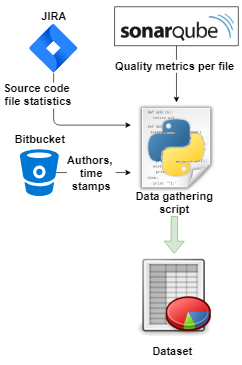
\includegraphics{\figpath/data_arch_small.png}
    \caption{Dataset Gathering operations}
    \label{fig:data_gathering}
\end{figure}

The first tool to be used in the data gathering process is Atlassian's JIRA server. JIRA is a ticketing system used by software developers to keep track of issues, feature requests and most importantly in the current context, bugs. Each ticket has been assigned a category upon its creation depicting its purpose. In the context of the current use case the most relevant types encountered are:

\begin{itemize}
    \item Story - represents a feature task to be done. Upon completion, it is a fully functional, testable vertical slice of functionality delivering value to end-users
    \item Task - represents an additional development task, such as, but not limited to, setting up test environments, automation of effort, including testing effort, infrastructure maintenance, etc. Does not provide direct value to end users
    \item Bug - represents issues found in released software, especially when expected and the actual behaviour of a given piece of functionality doesn't match.
\end{itemize}
Given that Task type tickets are not directly linked to the development life cycle they have been excluded from further analysis and the focus has been placed on Story and Bug type tickets instead.

The second use of the JIRA server was its proprietary integration with the source code repository - Bitbucket, as both tools are offered by the same company, Atlassian. For each of the JIRA tickets there existed a link between a given ticket and source code file changes, or commits, made and persisted in Bitbucket system. 
Each commit could consist of many files and each source code file could have been committed to multiple times under the umbrella of a single ticket. However, not all commit records under a ticket have been taken into the account - every so-called merge commit have been excluded.

To illustrate what a merge commit is and why it must be excluded \ref{fig:git-branching-merging-and-rebasing} will be used, where blue nodes signify the master or the golden copy of the code, and green and purple identify branches, where feature, bug fix or any other development work is carried out as part of a development lifecycle. At the end of its life, a branch will be integrated into the Master branch, which will generate a merge commit - illustrated by Feature branch. Additionally, it is a normal occurrence to have more than 1 branch created in a given codebase at any given time. If another branch has been created from the master before the Feature code was merged, as per \ref{fig:git-branching-merging-and-rebasing} Bug, and it is actively being developed on past the merge point such branch will have to be rebased. The rebase process will pull in the merge commit created by Feature, however, all source code files listed under merge commit will have already been analyzed under JIRA ticket representing the Feature, therefore should it not be excluded from the further analysis it would have duplicated the effort. Not excluding merge commits also represented significant risk with regards to story vs. bug categorization of source code files committed as Bug might as well have been a bug. In such scenario file committed under the Feature ticked would be categorized as non-bug, as per ticket category, as well as a bug as per category assigned by the second ticket.

\begin{figure}[!h]
    \centering
    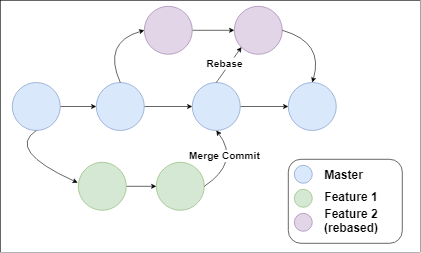
\includegraphics[scale=0.6]{\figpath/git_branching.png}
    \caption{GIT branching and rebasing strategy}
    \label{fig:git-branching-merging-and-rebasing}
\end{figure}

JIRA ticketing system provided the following columns:
\begin{itemize}
    \item issue key
    \item source repository
    \item file path
    \item category of the record, bug or not a bug
\end{itemize}

while the Bitbucket server provided additional information about:
\begin{itemize}\label{lst:design:info-from-bitbucket}
    \item author
    \item previous author
    \item commit timestamp
    \item timestamp of the previous commit
\end{itemize}

The final tool utilized was SonarQube by SonarSource, an open-source platform. Its capabilities include continuous inspection of code quality to perform automatic reviews with static analysis of code to detect code smells, reports on duplicated code, coding standards, unit tests, code coverage, code complexity, comments,  security vulnerabilities, and much more. In the context of this use case it was utilized to associate code metrics listed in Tables \ref{tbl:available-data-above-0-max-100} and \ref{tbl:available-data-above-0-no-max} as well as \files{}, \sqaleDebt{}, \statements{} and \violations{} provided in Table \ref{tbl:available-data-non-repeating-types}.

The \issueKey{}, \sourceRepository{} and \filePath{} were only used to verify that a given data point can be traced to a relevant JIRA ticket in order to verify it belongs to an assigned category, \authorAttrib{} and \prevAuthorAttrib{} were used to populate seniority and project tenure features. Finally, \timestamp{} and \prevTimestamp{} were used to calculate staleness of the file between changes.

\subsection{Machine Learning Models Utilized}

\subsubsection{Logistic Regression}
Logistic regression is a type of predictive analysis. It has been selected as it is considered an appropriate classification method when the target variable is binary\cite{Hastie2009OnLogisticRegForBinaryTargetClass}\cite{ridgeEstInLogReg}. 
As part of the analysis, two regularization methods were utilized to both reduce the number of features and to programmatically detect features contributing the most toward the correct classification of the target variable. 

\subsubsection{Linear Model Regularization} 
Regularization is defined as introducing an additional term to the loss function, the prediction model, in order to prevent overfitting of same. During the analysis Lasso and Ridge techniques, referred to as L1 and L2 regularization respectively, were used due to the number of features under analysis as both focus on coefficient shrinking, however, Table \ref{tab:regularization_l1_vs_l2} outlines key differences between the two methods, starting with the metrics measured by each.

\begin{table}[h!]
\centering
\begin{tabular}{@{}ll@{}}
\toprule
L1 & L2 \\ \midrule
Sum of weight & Sum of square of weights \\
Sparse outputs & Non-sparse output \\
Built-in feature selection & No feature selection \\
High sparsity for highly correlated features & \begin{tabular}[c]{@{}l@{}}Even coefficient distribution \\ for highly correlated features\end{tabular} \\
Can  interpret models with large feature sets & Main use case is preventing overfitting \\ \bottomrule
\end{tabular}
\caption{Summary of L1 vs L2 Regularization Techniques}
\label{tab:regularization_l1_vs_l2}
\end{table}

Both methods perform well in spite of the presence of correlated features: L1 by picking the most significant feature and zeroing the coefficient of the related features effectively excluding them from the prediction model, L2 by ensuring even distribution of the coefficients of the correlated features. 

Lasso stands for Least Absolute Shrinkage and it is defined as $RSS$ $+$ \textalpha{} $*$ (sum of absolute value of weights) or:
\begin{equation}\label{eq_lasso}
\sum^n_{i=1}(\hat{y_i}- y_i)^2 + \alpha \sum^n_{j=0}|w_j|
\end{equation}
where \textalpha{} refers to the factor of the penalty applied to a feature and $w_i$ refers to the weight of the feature\cite{Hastie2009SpringerOfLasso}.

Ridge regression works by adding a penalty factor to square of the magnitude of coefficients\cite{Hastie2009SpringerOfRidge}. It can be represented as:
\begin{equation}\label{eq_ridge}
\sum^n_{i=1}(\hat{y_i}- y_i)^2 + \alpha \sum^n_{j=0}w_j^2
\end{equation}
From the same definition it can be deducted that impact of \textalpha{} will be the same is both methods, namely:
\begin{enumerate}\label{list:impact-of-alpha}
\itemsep0em
\item\label{it:item1} $\alpha = 0$, is the same as linear regression, 
\item\label{it:item2} $\alpha = \infty$, the coefficients will be zero due to the infinite weighting on square coefficients anything less than 0 will make the objective infinite
\item\label{it:item3} $0 < \alpha < \infty$, the coefficients will be found between 0 and the ones obtained from a simple linear regression
\end{enumerate}

\subsubsection{Decision Tree Classifier}
Decision Tree for classification is a non-parametric method of supervised machine learning. Along with Decision Tree Regression, it was first proposed in 1984\cite{breimanCart1984} and it was intended as a top-down approach applied to a given set of data points. To find solutions a decision tree will make a number of sequential, hierarchical, or top-down, decisions about the outcome variable based on the predictor data. 

A very simplistic decision tree for classification has been represented in Figure \ref{fig:decision-tree-sample}. The tree is built top-down, starting from a root node corresponding to the best predictor for the dataset, which branches would extend downwards from. Going down the tree, depending on the position, the nodes would carry a different meaning. Terminal nodes, coloured in green, are points where no further decisions can be made, are called leaf nodes. The white nodes represent the decision boundary representing the points at which a classification rule, or classifier, is executed. The method serves in creating a consistent and standardized way of predicting what class should be applied to a given data point.

\begin{figure}[!h]
    \centering
    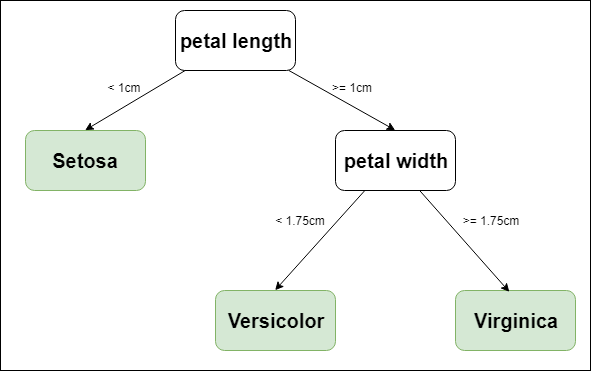
\includegraphics[scale=0.6]{Figures/decision_tree_sample.png}
    \caption{Sample Decision Tree Classification}
    \label{fig:decision-tree-sample}
\end{figure}

As the generation the tree progresses the classifiers are applied, depending on the features contained in the dataset, and continuously applied to each subset to generate additional nodes iteratively \cite{Bertsimas2017Cart} in each step while at the same time keeping track of the end structure of the tree. To an extent the method could be compared to a flowchart where no feedback loops are allowed, therefore making the model easy to explain as it is relatively easy to visualize the end structure of the tree, subject to the number of prediction-contributing features.

Given the mode of operation, the function implemented is step-wise, not linear, enabling the model to accommodate more complex relationships between the data. 
Additionally, it makes it less susceptible to the effects of feature collinearity, making it a highly valuable model candidate for datasets with high correlation factor values between features.

CART models, the decision tree classifier is part of, are models based purely on data from previous observations \cite{breimanCart1984} of a given target variable and no assumptions are made with regards to the distribution of errors or that of the data and it is considered a highly versatile model \cite{ensembleMethodsInMachineLearningDietterich} well able to explore the solution space without getting stuck in the local search optimum solution \cite{ensembleMethodsInMachineLearningDietterich}. However, at the same time, the model's reliance on previous observations indicates that the algorithm will terminate as soon as the optimal solution fitting the training data is found \cite{ensembleMethodsInMachineLearningDietterich} indicating that there is a possibility of an even more accurate solution to be devised in the future.

\subsection{Data Modelling}

Once a dataset has been generated as per section \ref{sec:design} it underwent the following operations:
\begin{enumerate}\label{lst:dataset-ops}
    \item missing data analysis and data cleaning \label{lst:dataset-ops.item:data-cleaning}
    \item balance of bug to non-bug records in the dataset \label{lst:dataset-ops.item:bug-to-non-bug-balance}
    \item outlier analysis \label{lst:dataset-ops.item:outliers}
    \item data correlation analysis \label{lst:dataset-ops.item:data-correlation}
    \item feature transformation \label{lst:dataset-ops.item:feature-transformation}
    \item data normalization \label{lst:dataset-ops.item:data-scaling}
    \item relevant feature selection \label{lst:dataset-ops.item:feature-selection}
    \item distribution of selected features \label{lst:dataset-ops.item:attribute-distribution}
    \item evaluation of regularized Logistic Regression model \label{lst:dataset-ops.item:ml-logistic-regression}
    \item evaluation of Decision Tree Classification model \label{lst:dataset-ops.item:ml-decision-tree}
    \item evaluation of additional models as necessary \label{lst:dataset-ops.item:ml-models-additional}
\end{enumerate}

Item \ref{lst:dataset-ops.item:data-cleaning} focuses on cleaning and imputing values for missing metrics. Item \ref{lst:dataset-ops.item:bug-to-non-bug-balance} will focus on listing the ratios between bug and non bug records in the dataset.
Item \ref{lst:dataset-ops.item:outliers} identifies if there are any projects or individual files that are diverging significantly from the rest of the dataset. 
Item \ref{lst:dataset-ops.item:data-correlation} focuses on identifying any feature correlation patterns in order to proceed with feature selection - item  \ref{lst:dataset-ops.item:feature-selection} after which it will be necessary to check for the balance and distribution of the selected features or attributes - which will be the focus of item \ref{lst:dataset-ops.item:attribute-distribution}. Feature distribution is included as part of the analysis as Logistic Regression model is susceptible to non-normally distributed datasets.
Item \ref{lst:dataset-ops.item:data-scaling} concentrates on evaluating multiple scaling methods with regards to their effectiveness of bringing the dataset values to the same scale of magnitude. The scaling method taken into the account are:
\begin{enumerate}
    \item Transformation using natural logarithm - $log(e)$ 
    \item Min-Max scaling
    \item Decimal Scaling Normalization (also referred to as Max-Abs scaling)
    \item Z-Score Normalization (also referred to as Standard scaling)
    \item Power Transformation using Yeo-Johnson method
    \item Quantile Transformation using uniform distribution variant
    \item Quantile Transformation using normal distribution variant
\end{enumerate}

Finally, an evaluation of the effectiveness of selected machine learning models with regards to predicting bug vs non-bug classes in the dataset will be carried out and constitutes the focus of items \ref{lst:dataset-ops.item:ml-logistic-regression}, \ref{lst:dataset-ops.item:ml-decision-tree} and \ref{lst:dataset-ops.item:ml-models-additional} respectively.
%%%%%%%%%%%%%%%%%%%%%%%%%%%%%%%%%%%%%%%%%%%%%%%%%%%%%%%%%%%%%%%%%%%%%%%%%%%%%%%%%%%%%%%%%
\subsubsection{Data Normalization methods}\label{sec:data-modelling:scalers}
\paragraph{Min Max method}\label{sec:data-modelling:scalers:min-max}
Min-max data normalization is a method of scaling data by assigning it a value in a range of between 0 and 1. Alternatively, the value range of -1 to 1 can also be used \cite{dataNormalization2014}. The method normalizes the values of the attributes of a data set according to the minimum and maximum values of a given attribute. The formula can be expressed as:
\begin{equation}\label{eq:min-max}
    \hat{a} = low+ \frac{(high - low)*(a - minA)}{maxA - minA)} 
\end{equation}
where $\hat{a}$ represents the transformed value of an attribute A.

It has been pointed out that this method suffers from uncertainty when normalizing time series data\cite{dataNormalization2014}, however, given that in this context it is not used to normalize time series value it has been included in the analysis.
\paragraph{Decimal Scaling}\label{sec:data-modelling:scalers:max-abs}
The decimal scaling normalization method works by scaling each feature by its maximum absolute value and can be represented by:
\begin{equation}
    \hat{a} = \frac{a}{10^d}
\end{equation}
where $\hat{a}$ represents the transformed value, $a$, the original value and $d$ is the smallest integer where $max(|\hat{a}|<1)$.

Similarly to min-max normalization, as this method also relies on knowing the maximum value of an attribute ahead of time, it has been unsuitable to time series data\cite{dataNormalization2014}. However, again, the attributes scaled do not include time series data it has been deemed appropriate to include it in the course of the analysis.

\paragraph{Z-Score Normalization}\label{sec:data-modelling:scalers:standard}
This method standardizes the features by removing the mean and scaling the attribute to unit variance. It can be represented y:
\begin{equation}
    \hat{a} = \frac{a - \mu(a)}{\sigma(a)}
\end{equation}
where $\hat{a}$ represents the transformed value, $\mu(a)$ is the arithmetic mean of a given attribute and $\sigma(a)$ is its standard deviation.

As this method does not rely on knowing the minimum and maximum values ahead of applying the transformation it overcomes the deficiencies of the Min-Max and Decimal Scaling methods\cite{dataNormalization2014}. However, at the same time, it faces difficulties with a non-stationary data series where the mean or standard deviation change over time.

\paragraph{Power Transformation - Yeo-Johnson method} \label{sec:data-modelling:scalers:power-yeo-johnson}
Power data normalization methods are a family of parametric, monotonic transformations aiming to alter given data from any distribution to as close to a Gaussian distribution as possible. As with any data normalization method, it is performed on data in order to reduce variance and minimize skewness.

The Box-Cox method,depicted in equation \ref{eq:box-cox} has been first proposed in 1964\cite{boxCox1964} and has been a very popular method of dealing with distribution variance \cite{YANG200614}. However, it is only applicable to strictly positive data\cite{YANG200614}. 
Additionally, as pointed out by Yeo and Johnson \cite{yeo-johnson-original} despite the fact that Box-Cox method could be modified to approximate normal distribution for negative $\lambda$, however, in those instances the proposed modifications fail when applied to heavily skewed distributions.
\begin{equation}\label{eq:box-cox}
    \hat{a}^{(\lambda)}=\begin{cases} \frac {{a}^{\lambda } - 1 }{\lambda}& \text{if $\lambda \neq 0$},\\
    ln(a)& \text{if $\lambda=0$}.
\end{cases}
\end{equation}

Provided the data is indeed heavily skewed, but despite the fact that all of the values present in the dataset are positive, as per the domain, the Box-Cox method has been ruled out as an appropriate data normalization method. Instead, Yeo-Johnson transformation, as per equation\ref{eq:yeo-johnson}, has been applied.

\begin{equation}\label{eq:yeo-johnson}
    \hat{a}^{(\lambda)}=\begin{cases} {\{{a +1}^{\lambda } - 1 }\}/ {\lambda}& \text{if $a \geq 0$ and $\lambda \neq 0$},\\
    log(a+1)& \text{if $a\geq 0$ and $\lambda=0$},\\
    -\{(-a +1)^\lambda -1\}/\lambda & \text{if $a < 0$ and $\lambda \neq 0$},\\
    -log(-a +1) & \text{if $a < 0$ and $\lambda = 0$}.
    
\end{cases}
\end{equation}

\paragraph{Quantile Transformation Methods} \label{sec:data-modelling:scalers:quantile}
Quantile regression has been deemed appropriate for heavily skewed data\cite{quantileNormalizationInSkewedDataAnalysis}, therefore, it has been included as part of the analysis.

The method is intended to spread out the most frequent data points for a given attribute, thus reducing the impact of marginal outliers.

There are two methods applied as part of the underlying analysis, the uniform and the normal distribution variants. The uniform distribution variant maps the data to a distribution with values between 0 and 1, spread out, as method name suggests, uniformly.

The normal distribution variant utilizes the mean and median of a given attribute where the median of the input becomes the mean of the output, centered at 0 value. 
%%%%%%%%%%%%%%%%%%%%%%%%%%%%%%%%%%%%%%%%%%%%%%%%%%%%%%%%%%%%%%%%%%%%%%%%%%%%%%%%%%%%%%%%%%%%%%%%%%%
\section{Implementation}\label{sec:implementation}
The implementation has been carried out in two steps. In the first step, a tool has been developed in Python language for the purpose of gathering the data required for the analysis - the process is outlined in Section \ref{sec:impl-data-gatherer}. Secondly, the data has been analyzed, in accordance with steps defined in Section \ref{sec:design}, List \ref{lst:dataset-ops}, using Jupyter Notebook tooling, which is the topic of Section \ref{sec:impl-data-analysis}.

%%%%%%%%%%%%%%%%%%%%%%%%%%%%%%%%%%%%%%%%%%%%%%%%%%%%%%%%%%%%%%%%%%%%%%%%%%%%%%%%%%%%%%%%%%%%%%%%%%%
\subsection{Data Gatherer}\label{sec:impl-data-gatherer}
The data gatherer tool has been split into a number of files for readability and maintenance. Additionally, a significant portion of the code written has been tested with automated tests to ensure the quality of the solution. Project structure is initially split between source code and test code folders, named \texttt{src} and \texttt{test} respectively. In each, a number of resource files have been defined to support the program execution, mock server responses, and data or provide additional information.

\begin{figure}[!h]
    \centering
    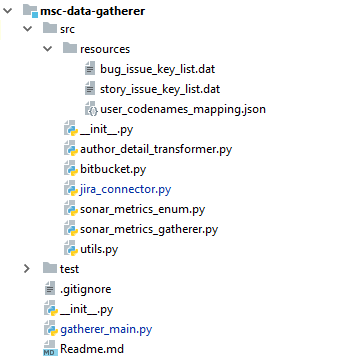
\includegraphics{Figures/impl_src_folder_files.png}
    \caption{Source Files Structure}
    \label{fig:impl-data-gatherer-source-files}
\end{figure}

The source folder structure has been illustrated in Figure \ref{fig:impl-data-gatherer-source-files} and it is comprised of the following elements:
\begin{enumerate}
    \item \texttt{gatherer\_main.py} - included in full in code excerpt \ref{code:gatherer_main.py}. Coordinates all data gathering operations. 
    \item\label{lst:impl.item:jira} \texttt{jira\_connector.py} - Handles all communication and authentication with a given JIRA server.
    \item\label{lst:impl.item:bitbucket} \texttt{bitbucket.py} - handles all communication and authentication with a given Bitbucket server.
    \item\label{lst:impl.item:sonar-metrics-gatherer} \texttt{sonar\_metrics\_gatherer.py} - is responsible for all communication via REST API with Sonar server instance.
    \item\label{lst:impl.item:author-encoder} \texttt{author\_detail\_transformer.py} is responsible for encoding authors' full names into code names to obfuscate sensitive identity details. 
\end{enumerate}

\subsubsection{Main Gatherer}\label{sec:source-code:main-gatherer}

\subsubsection{JIRA Connector}\label{sec:source-code:jira}
The very first operation that the JIRA connector class is responsible for is obtaining a list of JIRA keys. Typically composed of 3 to 4 letters, a key is an abbreviation uniquely identifying a given JIRA project. JIRA keys are obtained from a pre-compiled lists: the \texttt{bug\_issue\_key\_list.dat} and \texttt{story\_issue\_key\_list.dat} files, where the former contains only keys to Story-type tickets, while the latter to bug-type tickets. 
All of the communication with JIRA server happens over its publicly available REST API. In order to access it, base URL is required in the form of \mintinline{html}{<server_name>/jira/rest}.

The JIRA connector then interrogates the server by executing \mintinline{html}{/api/2/issue/{jira_key}} in order to obtain an ID attribute for each ticket. Ticket ID is a necessary parameter required in order to obtain the list of files committed under each ticket.

In the next step, a list of commits for a given JIRA ID is obtained for all code repositories from the \mintinline{html}{/dev-status/1.0/issue/detail?issueId={jira_id}&applicationType=stash} URL. The server response is in JSON format and as Figure \ref{fig:source-code:jira:commit-response} illustrates it is possible for any given commit to include multiple files, per repository. Additionally, many commits can be made under the same ticket, under many repositories. Based on Figure \ref{fig:source-code:jira:commit-response}, it should be assumed that the all of the next steps are executed for all files, under any commit in any repository provided by the above REST call.
\begin{figure}[!h]
    \centering
    \caption{Sample Response from JIRA detailing all commits made under given ticket}
    \label{fig:source-code:jira:commit-response}
    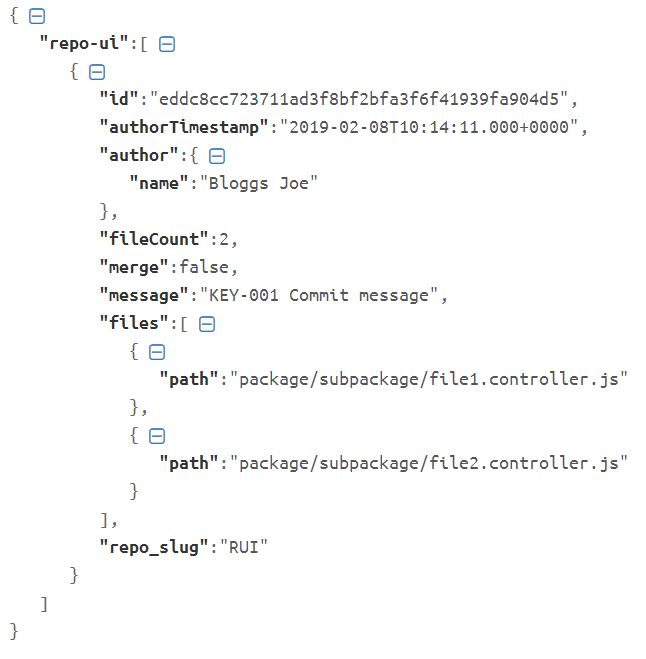
\includegraphics[scale=0.7]{Figures/gatherer/jira_connector_getting_commit_files_response.PNG}
    \caption{Caption}
    \label{fig:my_label}
\end{figure}
    
At this step, a number of infrastructure repositories that are maintenance-only, or ones that are written in languages not supported by Sonar server, thus making it impossible to obtain code quality metrics, have been removed. The repository names to be excluded are matched by a regular expression, from a list of static names compiled based on the domain knowledge of the infrastructure present at the business site. The repositories in question were mainly related to testing framework setup and maintenance, deployment pipelines for specific products and applications present at the business site or automated tests, etc. The list is not provided as it includes product names and it has been considered sensitive by the business owners.
    
In the next step, all merge commits are being removed from the analysis as it would otherwise create duplicate data points. For detailed explanation refer to Section \ref{sec:design}. 

Subsequently, a number of files are removed from the analysis - for listing of what file patterns were ignored, refer to Table \ref{tbl:file-extensions-excluded-from-analysis}. The files were excluded by name and/or extension pattern using regular expression and they represented a number of different categories detailed below. 

Firstly, "Test Files" column included the actual test classes housing the automated test scripts, their corresponding fixtures and object factories and any test configuration required by a given project.

The "Build and Infrastructure" column describes any files required, utilized or produced as part of a given project's build and publishing lifecycle. It also included any files relating to the infrastructure as code, which is heavily utilized in the applications under analysis to codify setup of any given deployment.

The third column, "Interfaces, Enums and Transfer Objects", details patterns for specific source code file for which code coverage doesn't exists as they're not strictly executable. This includes Java or Kotlin interface files, which as they do not have a specific file name associated with them, had to be compiled by trial and error and from own domain knowledge. Additionally, all of the enumerations in Java and Kotlin languages were excluded by utilizing the commonly applied "Enum" suffix. Furthermore, all data transfer object, which in the context of applications under analysis would only contain mutator methods, were excluded by utilizing the "Dto" suffix. 

The "Project Configuration" column refers to any configuration files contained in the project, which can refer to both application object setup, in the form of for example Spring Framework's Beans, as well as build tool files and properties. 
The "Other" column contains all of the files that did not fit any of the above categories. It represents the readme files, database scripts and other setup files.

To reiterate, all of the file patterns included in Table \ref{tbl:file-extensions-excluded-from-analysis} represent files for which no source code metrics could presently, be obtained from Sonar server. Therefore, they were removed to prevent generating noise in the analysis.


    
In the next and final step a list of initial metrics identifying a given commit is compiled. Alongside it, a map containing \texttt{issue\_key}, \texttt{source\_repository}, \texttt{commitId}, \texttt{path} and \texttt{repo\_code}, which is a unique 3-4 character abbreviation identifying a repository, is composed. Complete map containing both commit details as well as information necessary in the subsequent step is returned back to the coordinator file. 
    
For code listing for this step refer to code excerpt \ref{code:jira-connector.py}

\subsubsection{Bitbucket Connector}\label{sec:source-code:bitbucket}
Given data provided by JIRA server from above item interrogates a specified Bitbucket server over REST API in order to obtain details of the previous commit such as author and timestamp. As previously described in Section \ref{sec:design}, List \ref{lst:design:info-from-bitbucket} those details will be used in subsequent analysis steps to provide an indication of developers' level of experience based on seniority as well as familiarity with a given product based on the amount of time spent on the project.
    
Once all those details have been obtained and compiled they are returned to the coordinator file.
Complete code listing is available from code excerpt \ref{code:bitbucket.py}.
 
\subsubsection{Sonar Metrics Gatherer}\label{sec:source-code:sonar-metrics}
Using data gathered by JIRA and Bitbucket steps above it contacts Sonar server for each and every file, for each and every commit under each JIRA ticket and retrieves a specified list of code quality metrics. The list is defined in \texttt{sonar\_metrics\_enum.py} and it is comprehensive. 
    
In order to retrieve code quality metrics first, the expected parameters need to be generated from data retrieved from both JIRA and Bitbucket - the expected data is called project component and it is a unique identifier on Sonar Server for each file ever analyzed. The project component is in a different format for some projects, therefore, it was necessary to model a number of generation use cases, as outlined in the \texttt{sonar\_component\_name\_generator} method in \ref{code:sonar-gatherer.py} code listing.
    
One thing of note is that for different source code languages different metrics, especially with regards to the code coverage metrics can be provided by Sonar. For example, for JavaScript-based languages such as Angular JS there is a separate position for integration, or IT, coverage, whereas for Java and other JVM based languages that metric is rarely provided. In JVM based languages it has been folded into the \texttt{overall code coverage} metric instead.


\subsubsection{Author Detail Transformer}\label{sec:source-code:author-encoder}
it is invoked after code quality metrics have been gathered by \texttt{SonarMetricsGatherer} class.

\subsubsection{Other Utilities}


\begin{table}[h!]
\centering
\caption{Files excluded from the analysis by extension or suffix}
\label{tbl:file-extensions-excluded-from-analysis}
% \begin{tabular}{@{}llll@{}}
% \toprule
% \multicolumn{4}{c}{Exclusion Patterns} \\ \midrule
% .*Test.*.java & .*Interface.*\textbackslash{}.java & .*NameToIndex\textbackslash{}.java & .*\textbackslash{}.jar \\
% .*Test.*.kt & .*Interface.*\textbackslash{}.kt & .*Config.kt & .*Dto.*kt \\
% .*\textbackslash{}.e2e-spec.js & .*\textbackslash{}.stub.js & .*\textbackslash{}.po.js & .*spec.js \\
% .*\textbackslash{}.ico & .*\textbackslash{}.npmrc & .*\textbackslash{}.conf.js & .*gulpfile.js \\
% .*ColumnDef.js & .*Spec.js & .*Decorator.js & \textbackslash{}.eslintrc \\
% .*\textbackslash{}.gitattributes & .*\textbackslash{}.sql & .*\textbackslash{}.csv & .*\textbackslash{}.xlsx \\
% .*\textbackslash{}.txt & .*\textbackslash{}.xlsm & .*\textbackslash{}.yaml & .*\textbackslash{}.yml \\
% .*WriteService.* & .*DeleteService.* & .*CreateService.* & .*\textbackslash{}.lock \\
% .*.gradle & .*\textbackslash{}.?factory.js & .*\textbackslash{}.css & .*.config.js \\
% .*Config.java & .*\textbackslash{}.html & .*\textbackslash{}.svg & .*ColumnDefs.js \\
% .*\textbackslash{}.gz & .*ReadService.* & \textbackslash{}.gitignore & .*\textbackslash{}.json \\
% .*\textbackslash{}.war & .*Enum.*kt & .*\textbackslash{}.scss & .*factories.js \\
% .*Jenkinsfile.* & .*\textbackslash{}.xml & .*\textbackslash{}.md & .*\textbackslash{}.properties \\ \bottomrule
% \end{tabular}

\begin{tabular}{@{}lllll@{}}
\toprule
Test Files & \begin{tabular}[c]{@{}l@{}}Build and Deployment \\ infrastructure\end{tabular} & \begin{tabular}[c]{@{}l@{}}Interfaces, Enums \\ and Transfer Objects\end{tabular} & Project configuration & Other \\ \midrule
.*Test.*.java & .*\textbackslash{}.war & .*Interface.*\textbackslash{}.java & .*Config.java & .*\textbackslash{}.csv \\
.*Test.*.kt & .*Jenkinsfile.* & .*Interface.*\textbackslash{}.kt & .*Config.kt & .*\textbackslash{}.css \\
.*\textbackslash{}.e2e-spec.js & .*\textbackslash{}.jar & .*ReadService.* & .*.config.js & .*\textbackslash{}.svg \\
.*\textbackslash{}.stub.js & .*\textbackslash{}.npmrc & .*Enum.*kt & .*.gradle & .*\textbackslash{}.scss \\
.*Spec.js & .*\textbackslash{}.yml & .*NameToIndex\textbackslash{}.java & \textbackslash{}.gitignore & .*\textbackslash{}.md \\
.*\textbackslash{}.?factory.js & .*\textbackslash{}.lock & .*CreateService.* & .*\textbackslash{}.gitattributes & .*\textbackslash{}.json \\
.*\textbackslash{}.po.js & .*gulpfile.js & .*WriteService.* & .*\textbackslash{}.properties & .*\textbackslash{}.xlsx \\
.*spec.js & \textbackslash{}.eslintrc & .*DeleteService.* &  & .*\textbackslash{}.ico \\
.*ColumnDefs.js & .*\textbackslash{}.conf.js & .*Dto.*kt &  & .*\textbackslash{}.txt \\
.*factories.js & .*\textbackslash{}.yaml & .*Decorator.js &  & .*\textbackslash{}.gz \\
.*ColumnDef.js &  &  &  & .*\textbackslash{}.sql \\
 &  &  &  & .*\textbackslash{}.xlsm \\
 &  &  &  & .*\textbackslash{}.html \\
 &  &  &  & .*\textbackslash{}.xml \\ \bottomrule
\end{tabular}
\end{table}




\begin{landscape}

\begin{code}
\captionof{listing}{Main data gathering component - the coordinator}
\label{code:gatherer_main.py}
\inputminted{python}{source_code/gatherer.py}
\end{code}

\begin{code}
\captionof{listing}{JIRA Connector - extracts relevant metrics from a given JIRA ticket}
\label{code:jira-connector.py}
% \begin{minted}[breaklines]{python}
\inputminted{python}{source_code/jira_connector.py}
% \end{minted}
\end{code}

\begin{code}
 \captionof{listing}{Bitbucket connector - retrieves commit metrics for a given file}
 \label{code:bitbucket.py}
\inputminted{python}{source_code/bitbucket_connector.py}
 \end{code}
 
 \begin{code}
 \captionof{listing}{Sonar connector - retrieves code quality metrics for a given file}
 \label{code:sonar-gatherer.py}
 
 \inputminted{python}{source_code/SonarMetricsGatherer.py}
 
 \end{code}

\end{landscape}


\subsection{Data Analysis Implementation}\label{sec:impl-data-analysis}
\subsubsection{Initial Dataset Analysis}
Initial analysis of the dataset constructed in section \ref{sec:impl-data-gatherer} revealed that it's comprised of 6547 rows spread across 67 columns, where each column corresponds to a feature. Out of the 67 columns, the vast majority is of numeric type, with only 5 being a text and 1, the prediction target column, referred to as \texttt{is\_bug} being of type boolean.

\subsubsection{Timestamps features transformation}\label{sec:impl-data-analysis:make-file-age}
As previously mentioned in section \ref{sec:data-available} the \timestamp{} and \prevTimestamp{} representing the time the current file commit was made as well as the last time commit has been made to the file had to be transformed into a single column outlining the age of the file - determining the staleness of it.
During the transformation, it has been discovered that in 7 instances the resulting column took on a negative value. This should have been impossible and as such, each case was investigated and verified against source data contained in Bitbucket server, as per section \ref{sec:data-available}. In all 7 cases, the actual data gathered from the Bitbucket server has been incorrect at the source. Given that short of manually gathering timestamps and correcting previous author data, there is no way to recover as well as the fact that such error occurred only in 7 records it was deemed best to removed them.
At the end of the transformation \timestamp{} and \prevTimestamp{} columns were removed, changing the shape of the dataset to 66 columns instead of initial 67.

\subsubsection{Files deleted}\label{sec:impl-data-analysis:files-deleted}
Progressively, an analysis of any missing values from all the columns was conducted. The first step was to determine if any of the files committed to having since been deleted. It has been determined by using the \files column provided by Sonar server. If the value of the column was not equal to 1 then such file no longer existed in the repository, despite the presence of historical code metrics. As a result, 431 rows were removed from the dataset. It should be noted that it doesn't mean that 431 different files were removed from the dataset as any file could have been committed to multiple times as each such commit would be represented by a row in the dataset. The obsolete file removal left the dataset at 6109 rows in 66 columns.

\subsubsection{Columns with all values at 0}\label{sec:impl-data-analysis:all-cols-at-0}
Next step was to check if there were any features present where all values were at 0 value. It has been determined that a column where all values are of 0 value would not contribute towards the prediction and therefore can be removed. The list of 19 removed columns is presented in Table \ref{tbl:zero-value-columns}. This step left the dataset with 6109 rows and 47 columns.

\begin{table}[h!]
\centering
\caption{Columns with all values at 0}
\label{tbl:zero-value-columns}
\begin{tabular}{@{}ll@{}}
\toprule
Column Name & Column Name \\ \midrule
blocker\_violations & public\_undocumented\_api \\
bugs & reliability\_remediation\_effort \\
confirmed\_issues & reopened\_issues \\
critical\_violations & security\_remediation\_effort \\
effort\_to\_reach\_maintainability\_rating\_a & skipped\_tests \\
false\_positive\_issues & test\_errors \\
generated\_lines & test\_failures \\
generated\_ncloc & vulnerabilities \\
it\_coverage & wont\_fix\_issue \\
it\_line\_coverage &  \\ \bottomrule
\end{tabular}
\end{table}



\subsubsection{Missing or negative values}\label{sec:impl-data-analysis:missing-or-negative-values}
Subsequently, an investigation into any values missing from any columns was investigated. The findings were summarized in Table \ref{tbl:missing-values-per-col}, with 13 columns showing a number of values missing. The missing values were then filled with the median per column, as per code listing \ref{code:missing-values-median-code}. Filling missing values with the median as opposed to mean metric has been preferred due to a large variance of some of the columns. In such instance it is more reliable to impute missing values from the median as mean is susceptible to extreme values - indicated by large variance values. It can be observed in Figure \ref{fig:high-variance} the variance distribution across columns - note that only columns with variance exceeding 100 have been included. Additionally, the \fileAgeInSec{} column has been removed as its variance value of approximately 0.5 billion would have skewed the graph making other properties unreadable. File age's variance is almost 17 times larger given that second largest variance of approximately 30000 belonging to \lines{} column.

\begin{code}
\captionof{listing}{Missing Values Filled per Column}
\label{code:missing-values-median-code}
\begin{minted}[breaklines]{python}
for col in cols:
        df[col] = df[col].fillna(df[col].median())
\end{minted}
\end{code}

\begin{figure}[h!]
    \centering
    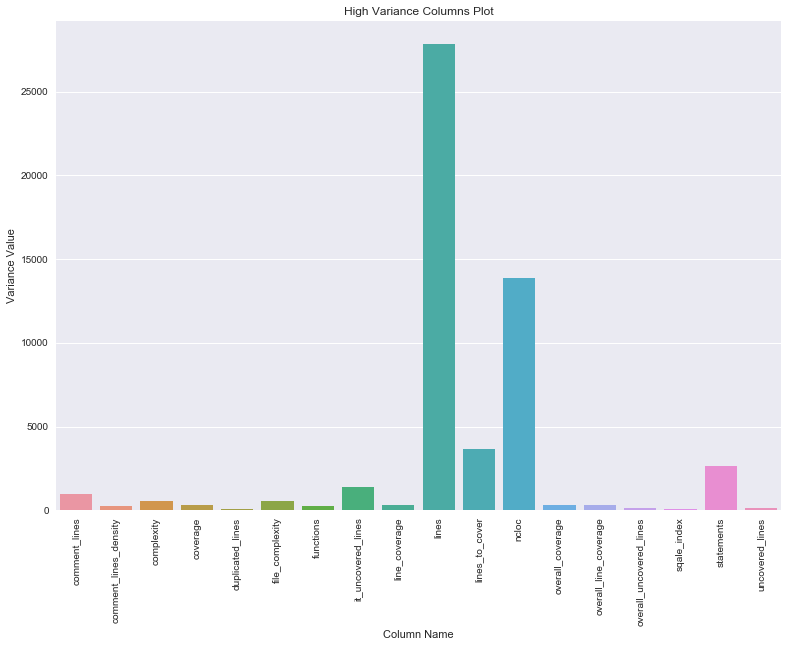
\includegraphics[scale=0.6]{\figpath/High_Variance_Columns_Plot.png}
    \caption{Attributes with high variance}
    \label{fig:high-variance}
\end{figure}

\begin{table}[h!]
\centering
\caption{Missing Values per Column}
\label{tbl:missing-values-per-col}
\begin{tabular}{@{}ll@{}}
\toprule
Column Name & No of missing values \\ \midrule
branch\_coverage & 2551 \\
coverage & 637 \\
function\_complexity & 119 \\
it\_uncovered\_lines & 3890 \\
line\_coverage & 637 \\
lines\_to\_cover & 637 \\
overall\_branch\_coverage & 2551 \\
overall\_coverage & 637 \\
overall\_line\_coverage & 637 \\
overall\_uncovered\_conditions & 2551 \\
overall\_uncovered\_lines & 637 \\
uncovered\_conditions & 2551 \\
uncovered\_lines & 637 \\ \bottomrule
\end{tabular}
\end{table}
\FloatBarrier

\subsubsection{Determining class balance} \label{sec:impl-data-analysis:class-balance}
Once the data has been cleaned and all missing values were filled, the next step was to determine the balance between values for the target class \isBug{}. It has been determined that the number of bug records was, 742, or approximately 12.15\% whereas non-bug records comprised of 5367, or approximately 87.85\%. As such the bug class was severely undersampled. Class balance has been conducted by checking how many rows in the dataset have had \texttt{True} value in the \isBug{} feature and how many were associated with \texttt{False} value, as per code snippet \ref{code:class-balance-impl}. The reasoning behind not just subtracting the number of \texttt{True} labels from the total row count of the dataset was to catch any rows that had neither label associated with them. 

Given the steps undertaken it has been proven beyond doubt that all data samples have a value for \isBug{} feature, with data points categorized as \texttt{bug} being severely undersampled.

\subsubsection{Resampling the classes}\label{sec:impl-data-analysis:resampling}
Upsampling and downsampling techniques have both been investigated and implemented as part of the analysis. The downsampling method will randomly remove records from majority class while the upsampling method will randomly duplicate minority class records in order to reach balance between classes in the prediction target feature \isBug{}. 

In order for the process to be implemented first the determination into which class is in the majority and which in the minority had to be conducted. It has been implemented similarly to checking the class balance from code excerpt \ref{code:class-balance-impl}, however, instead of collecting values into lists by their indices, they are separated into 2 data frames, one for \texttt{True} and one for \texttt{False} classes. Then a determination into which of these data frames will be treated as majority and which is the representation of the minority class. At the end of the process data frames representing same are returned from the function for further processing, with complete code definition being available in excerpt \ref{code:class-separation-impl}

Subsequently, the resampling of either class is conducted via \texttt{resample} function provided by sci-kit learn package. Said function takes in the following parameters:
\begin{itemize}
    \item data frame to be resampled. In case of upsampling it is the dataframe containing all of the the minority class records and in case of downsampling it is the dataframe representing the majority class.
    \item replace parameter takes in a boolean value. It is set to \texttt{True} for upsampling operation and \texttt{False} for the downsampling
    \item the number of records the minority or majority class needs to be resampled to. In case of psamplng this will be the number of records contained in the majority class and in case of downsampling it will match the number of records in the minority class dataframe
    \item random state parameter - given that resampling operation is random by nature, the records are either randomly duplicated, upsampling, or deleted, downsampling, there is a need to ensure the same results between different executions of the complete analysis. That consistency is secured by providing the same number to the \texttt{random\_state} parameter. The value of the parameter is irrelevant, as long as it is provided.
\end{itemize}

In the last step dataframes representing the majority and minority, now resampled, are combined into to forma single dataframe representing the dataset and returned for further analysis.


For complete source code listing refer to sample \ref{code:resampling-impl}.


\subsubsection{Feature Distribution}\label{sec:impl-data-analysis:feature-dist}
\todo{fill it out}

\subsubsection{Outliers}\label{sec:impl-data-analysis:outliers}

\subsubsection{Data Correlation}\label{sec:impl-data-analysis:corr:generic-approach}
The following section will focus on identifying data correlation between features present in the dataset. The methods employed will be both numerical and visual. A numerical method has been employed for brevity and as verification for the visual method as it believed that with 40+ features it will be quite cumbersome to distinguish between high and low correlation values in a matrix.

\begin{figure}
    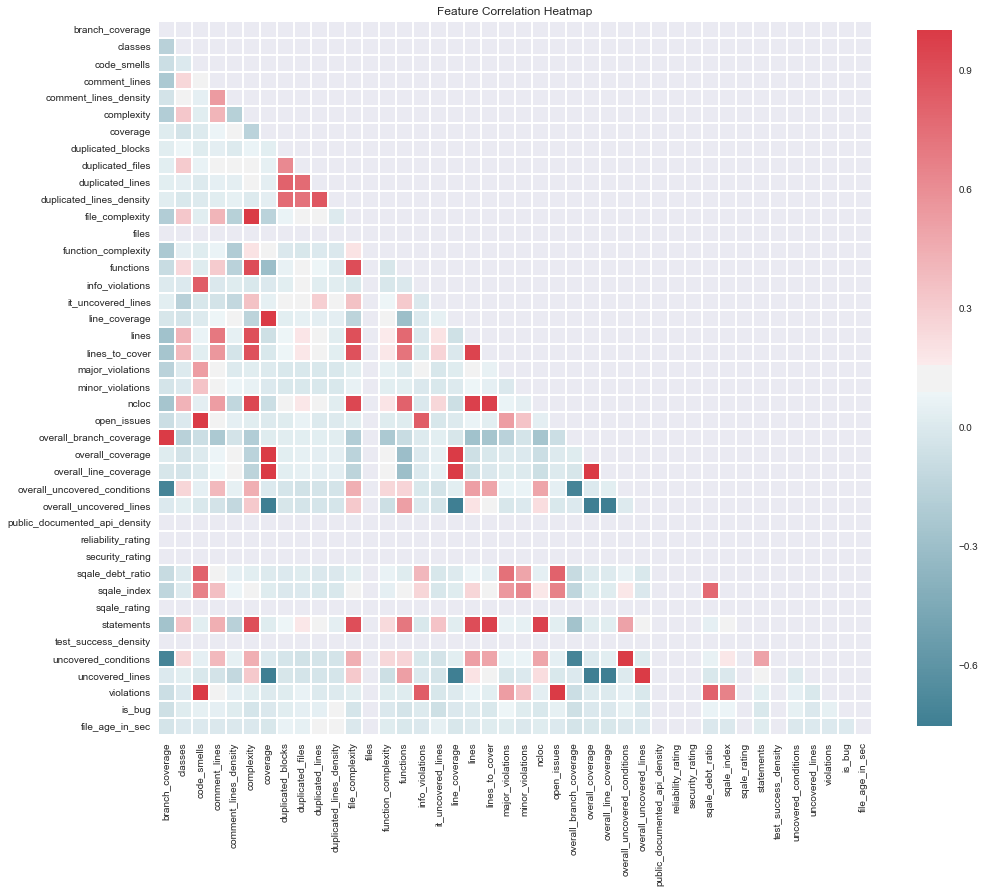
\includegraphics[scale=0.5,left]{\figCorrPath/Feature_Correlation_Heatmap.png}
    \caption{Feature Correlation Heatmap}
    \label{fig:correlation-all-features}
\end{figure}


The heatmap illustrated in Figure \ref{fig:correlation-all-features} served as a method of selecting candidates for:
\begin{itemize}
    \item feature transformation, where features with high positive correlation factor may be combined 
    \item selecting candidates from non-correlated features for visualizing how their values change in relation to one another
\end{itemize}

Unfortunately, the same figure was too large and involved to determine likely candidates visually, therefore it was decided to break it up into a number of smaller, subsection graphs. Features for the subsection graphs were selected based on name similarity or, based on previously acquired domain, similar metrics.
Therefore the most approach decided on was to split the correlation heatmap into subplots containing similar metrics, which was expected to produce a number of candidates for feature transformation. In order to decide how to transform feature candidates listed the following steps were undertaken in all cases:
\begin{enumerate}
    \item scatter plot depicting the relationship between the candidates
    \item the distribution of values 
    \item deciding on transformation approach, e.g. deletion, combination, etc
\end{enumerate}

Each heatmap was generated using the same implementation, as per code snippet \ref{code:corr-heatmap-impl} utilizing output of correlation function provided by Pandas DataFrame via \texttt{df.corr()} function. Said function provides a numerical metric of correlation between the attributes provided in the data frame. Should the value be positive then a positive correlation is present, meaning that an increase in one value will result in an increase, not necessarily of the same magnitude, in the corresponding metric. The opposite is true for metrics where the correlation factor is negative. The absolute value of the correlation factor represents the strength of the correlation with the greater value indicating a stronger relationship. Correlation factor near 0 is indicative of independence between attributes.

Each scatter plot between a pair of attributes has been implemented using code snippet \ref{code:line-scatter-plot-impl}, where the $x$ and $y$ parameters refer to feature names and \texttt{data} parameter is supplied with the dataframe representing the complete dataset.

\begin{code}
\captionof{listing}{Scatter Plot Between 2 Features - Implementation}
\label{code:line-scatter-plot-impl}
\begin{minted}[breaklines]{python}
sb.lmplot(x=column1, y=column2, truncate=True, size=5, data=dataFrame)
\end{minted}
\end{code}

More complex scatterplots, those between multiple attributes have been implemented using excerpt \ref{code:feat-transf:scatterplot}, where \texttt{data} is the complete dataset, \texttt{vars} is an array of column names to be include in the graph, \texttt{diag\_kind} is the kind of the diagram to be generated, between kernel density estimation plot or a histogram.
\begin{code}
\captionof{listing}{Scatter Plot Between Multiple Features - Implementation}
\label{code:feat-transf:scatterplot}
\begin{minted}[breaklines]{python}
sb.pairplot(data=df, vars =[column1, column2, column3, column4], diag_kind = 'kde', size=3)
\end{minted}
\end{code}

The distribution of attributes under analysis has been plotted on a single plane in a graph and has been implemented as depicted in code snippet \ref{code:feat-transf:distribution-multiplot}. It should be noted that the code has not been made generic to accommodate a variable number of attributes and is only suited for depicting pairs of attributes. To accommodate multiple attributes 2 places would have to be updated: the number of colours in the \texttt{colours} array would have to correspond to the number of attributes under analysis. The names of available colours can be found in Seaborn library's documentation. The second modification would have had to be made to the number of \texttt{sb.distplot(....)} calls - one call should be made for each attribute distribution to be plotted.

Alternatively, an additional method for depicting the relationship between attributes on three-dimensional space has been devised as per snippet \ref{code:feat-transf:3d-graph-impl}.

\FloatBarrier

%%%%%%%%%%%%%%%%%%%%%%%%%%%%%%%%%%%%%%%%%%%%%%%%%%%%%%%%%%%%%%%%%%%%%%%%%%%%%%%%%%%%%%%%%%%%%%%%%%%%%%%%%%%%%%%
\paragraph{Code Coverage Related Metrics}\label{sec:impl-data-analysis:corr:code-coverage}
The first subplot to be analyzed was populated with features relating to code coverage metrics:
\begin{itemize}\label{lst:code-coverage-candidates}
    \item \branchCoverage{}
    \item \overallBranchCoverage{}
    \item \overallCoverage{}
    \item \overallLineCoverage{}
    \item \overallUncoveredConditions{}
    \item \overallUncoveredLines{}
    \item \coverage{}
    \item \lineCoverage{}
    \item \uncoveredConditions{}
    \item \uncoveredLines{}
\end{itemize}
and it's correlation statistics can be observed in Figure \ref{fig:correlation-coverage-metrics-subplot}. From the same graph, 4 candidates for feature transformation into a single feature due to high positive correlation with one another can be identified:
\begin{enumerate}\label{lst:corr-sub:code-coverage-transf-candidates}
    \item \overallBranchCoverage{} and \branchCoverage{}
    \item \overallUncoveredLines{} and \uncoveredLines{}
    \item \overallCoverage{}, \overallLineCoverage{}, \coverage{} and \lineCoverage{}
    \item \overallUncoveredConditions and \uncoveredConditions{}
\suspend{enumerate}

\begin{figure}[h!]
    \centering
    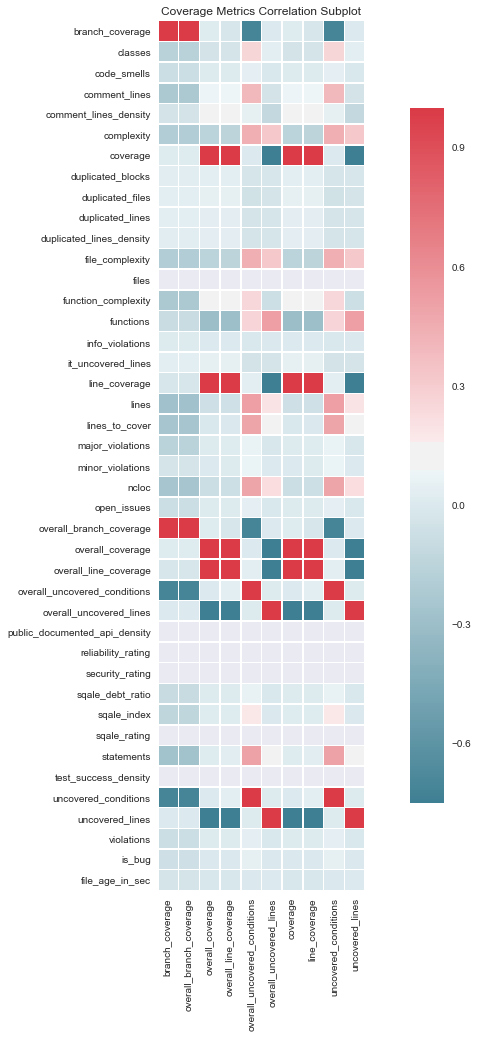
\includegraphics[scale=0.7]{\figCorrPath/Coverage_Metrics_Correlation_Subplot.png}
    \caption{Code Coverage Metrics Correlation Subplot}
    \label{fig:correlation-coverage-metrics-subplot}
\end{figure}
\FloatBarrier

Based on the scatter plot, generated from using code excerpt \ref{code:feat-transf:scatterplot}, depicted in Figure \ref{fig:candidate1-scatterplot} constructed for the transformation Candidate 1 listed above, it is thought that the attributes have a positive, almost perfectly linear relationship between one another, meaning that as one attribute increases in value so does the corresponding one, furthermore the increase or decrease in value is of the same magnitude.
\begin{figure}[h!]
    \centering
    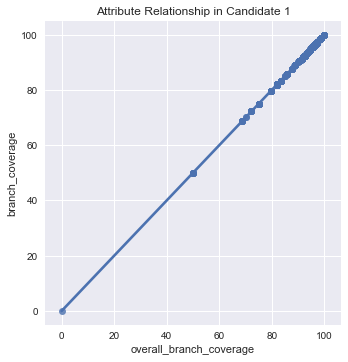
\includegraphics[scale=0.9]{\figCorrPath/Attribute_Relationship_in_Candidate_1.png}
    \caption{Relationship between \overallBranchCoverage{} and \branchCoverage{} attributes}
    \label{fig:candidate1-scatterplot}
\end{figure}

From the Figure \ref{fig:candidate1-distribution}, implemented by code snippet \ref{code:feat-transf:distribution-multiplot}, it can be surmised that the distribution of values for both attributes is perfectly aligned. To ascertain that claim an individual graph was plotted just for the invisible attribute \overallBranchCoverage{} which can be observed in Figure \ref{fig:candidate1-attrib2-distribution}.
From the investigation conducted it was deemed fair to conclude that it doesn't matter which attribute is preferred to be retained for Candidate 1 - \overallBranchCoverage{} or \branchCoverage{} as their values were almost identical. Based on the attribute name the column representing the overall coverage was selected to remain while the other was to be removed.

\begin{landscape}
\begin{figure}
\centering
\begin{minipage}{0.89\textwidth}
  \centering
  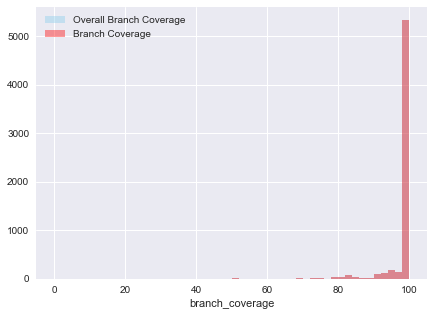
\includegraphics[scale=0.7]{\figCorrPath/Attribute_Distribution_in_Candidate_1.png}
    \caption{Distribution of \overallBranchCoverage{} and \branchCoverage{} attributes}
    \label{fig:candidate1-distribution}
\end{minipage}%
\begin{minipage}{0.89\textwidth}
   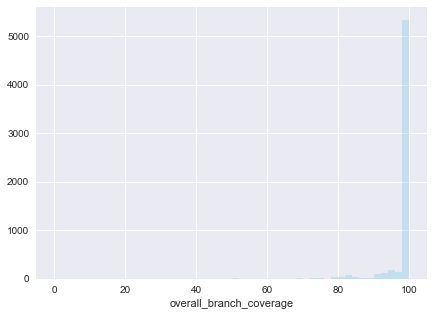
\includegraphics[scale=0.7]{\figCorrPath/Attribute_Distribution_in_overall_branch_coverage.png}
    \caption{Distribution of \overallBranchCoverage{} attribute}
    \label{fig:candidate1-attrib2-distribution}
\end{minipage}
\end{figure}
\end{landscape}
\FloatBarrier

Candidate 2 analysis started with the charting of a scatter plot for the selected attributes, the \overallUncoveredLines{} and \uncoveredLines{}, presented in Figure \ref{fig:candidate2-scatterplot}, and as with Candidate 1 displayed a positive linear relationship between the data points, with the majority of data focused close to 0 value.

\begin{figure}[h!]
    \centering
    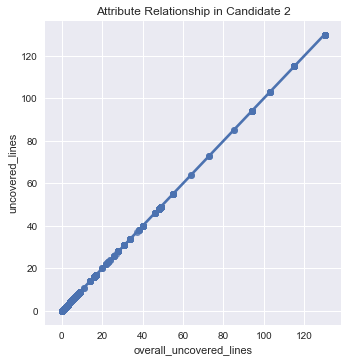
\includegraphics[scale=0.9]{\figCorrPath/Attribute_Relationship_in_Candidate_2.png}
    \caption{Relationship between \overallUncoveredLines{} and \uncoveredLines{} attributes}
    \label{fig:candidate2-scatterplot}
\end{figure}

The distribution of the \overallUncoveredLines{} and \uncoveredLines{} is the same as per Figure \ref{fig:candidate2-distribution}. Since it has been previously illustrated that when only 1 graph line is visible it is in fact perfectly overlain over the distribution line for the other attribute in the analysis of Candidate 1, therefore, a special graph depicting the distribution of \uncoveredLines{} will not be provided.
\begin{figure}
    \centering
  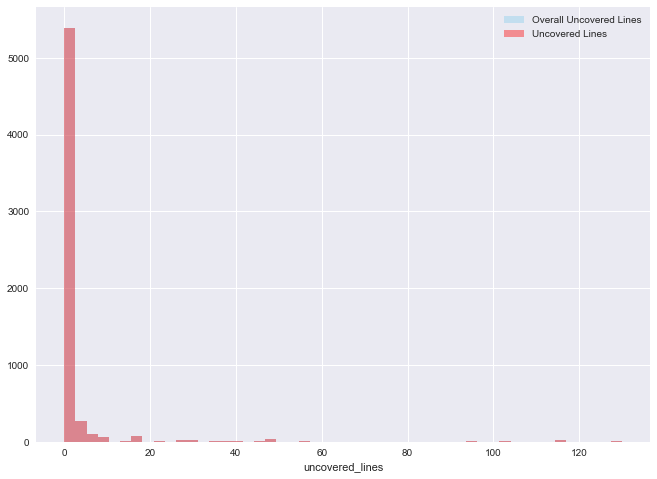
\includegraphics[scale=0.7]{\figCorrPath/Attribute_Distribution_in_Candidate_2.png}
    \caption{Distribution of \overallUncoveredLines{} and \uncoveredLines{} attributes}
    \label{fig:candidate2-distribution}
\end{figure}
In case of Candidate 2 it  has been decided to retain \overallUncoveredLines{} attribute as using domain knowledge of the metrics it stood to reason that this attribute would be more encompassing than \uncoveredLines{}.
\FloatBarrier

Given the depiction of both the linear relationship between the multiple  attributes of \overallCoverage{}, \overallLineCoverage{},\coverage{} and \lineCoverage{}, presented in Figure \ref{fig:candidate3-pairplot} and the distribution, provide on the diagonal it was summarily concluded that the attributes follow the same trends and only one of the four should be retained. Therefore, based on previous domain knowledge of the metrics \overallCoverage{} was deemed the most encompassing and has been retained.
\todo{the pair plot needs an update of the title as it's not distribution. Plus need to plot distributions as pair plot diagonal is NOT a representation of distribution}
\begin{figure}[h!]
    \centering
    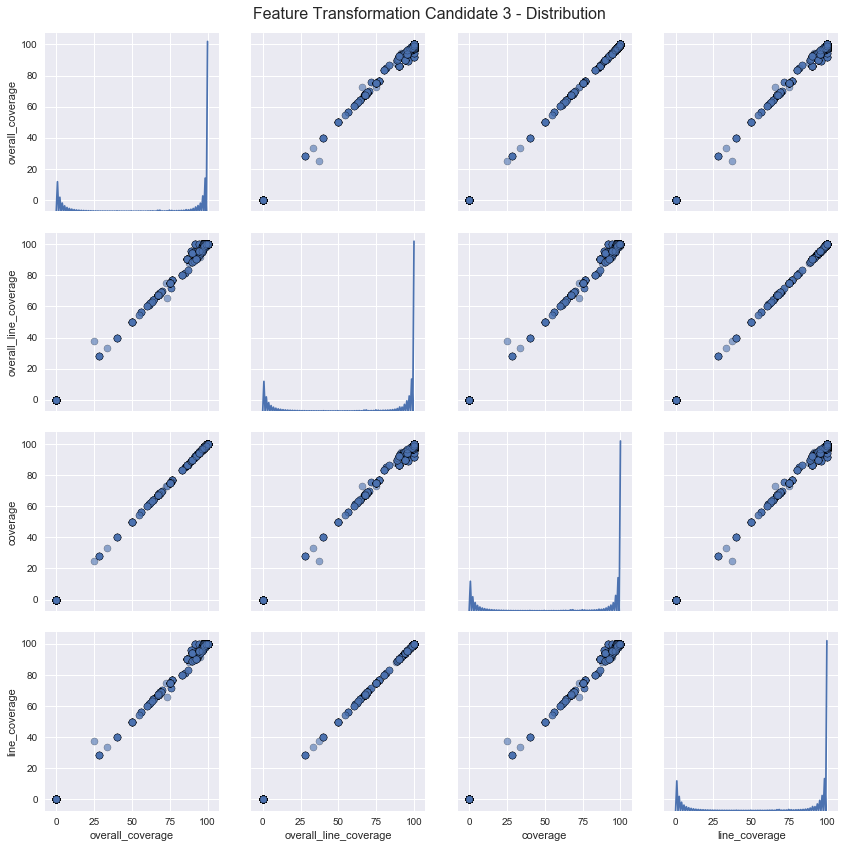
\includegraphics[scale=0.5]{\figCorrPath/Attribute_Relationship_in_Candidate_3.png}
    \caption{Relationship between multiple attributes}
    \label{fig:candidate3-pairplot}
\end{figure}

\FloatBarrier

The last feature transformation will be conducted between \overallUncoveredConditions{} and \uncoveredConditions{} attributes. In Figure \ref{fig:candidate4-scatterplot} it can be observed a perfectly linear relationship between the two attributes under investigation. Additionally, a change in one attribute corresponds directly to an increase of the corresponding attribute not only in the direction of the change but also in the magnitude. Furthermore, from Figure \ref{fig:candidate4-distribution} again a perfectly aligned distribution of both attributes can be observed leading to a conclusion that the attributes under question are equivalent.

\begin{figure}[h!]
    \centering
    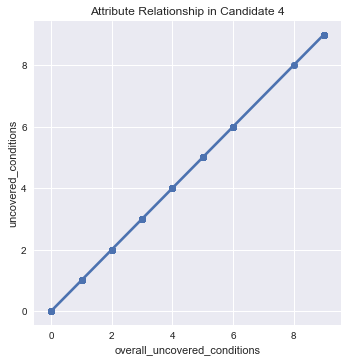
\includegraphics[scale=0.7]{\figCorrPath/Attribute_Relationship_in_Candidate_4.png}
    \caption{Relationship between \overallUncoveredConditions{} and \uncoveredConditions{} attributes}
    \label{fig:candidate4-scatterplot}
\end{figure}

\begin{figure}[h!]
    \centering
    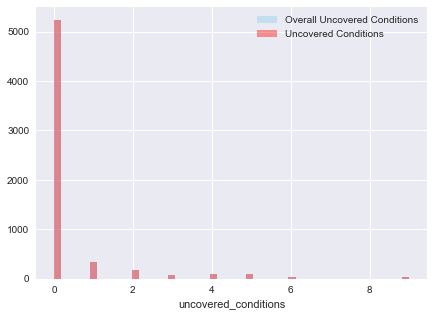
\includegraphics{\figCorrPath/Attribute_Distribution_in_Candidate_4.png}
    \caption{Distribution of \overallUncoveredConditions{} and \uncoveredConditions{} attributes}
    \label{fig:candidate4-distribution}
\end{figure}

\FloatBarrier
%%%%%%%%%%%%%%%%%%%%%%%%%5
\textbf{In conclusion} all features investigated in this section have displayed high positive relationship with one another, very strong linear relationship as well as almost perfectly aligned data distribution. Therefore, only 4 of the 10 attributes, enumerated in section \ref{lst:code-coverage-candidates}, have been retained:

\begin{itemize}
    \item \overallBranchCoverage{}
    \item \overallUncoveredLines{}
    \item \overallCoverage{}
    \item \overallUncoveredConditions{}
\end{itemize}

\paragraph{Line and complexity features}\label{sec:impl-data-analysis:corr:line-and-complexity}
In the following section, a number off attributes will be investigated with regards to the possibility of transforming said features and reducing the dimensionality of the overall dataset. Given a subplot of a heatmap presented in Figure \ref{fig:correlation-line-metrics-subplot} the attributes under analysis are, based on their high correlation:
\resume{enumerate}
    \item \complexity{}, \fileComplexity{}    \item \statements{}, \linesToCover{}
    \item \ncloc{}, \lines{}
\suspend{enumerate}
It is worth noting that despite similar naming \functionComplexity{} metric does not display a strong correlation with the other two complexity metrics and was not included  as part of Candidate 5.

The numbering of feature transformation candidates is being continued from the previous section, where candidates 1 through 4 were discussed.

Starting with Candidate 5, in Figure \ref{fig:candidate5-pairplot}, it can be observed that \complexity{} and \fileComplexity{} have an outstandingly well defined linear relationship. The attribute distribution also follows the same pattern, with a highly pronounced left tail. 

\begin{figure}
    \centering
    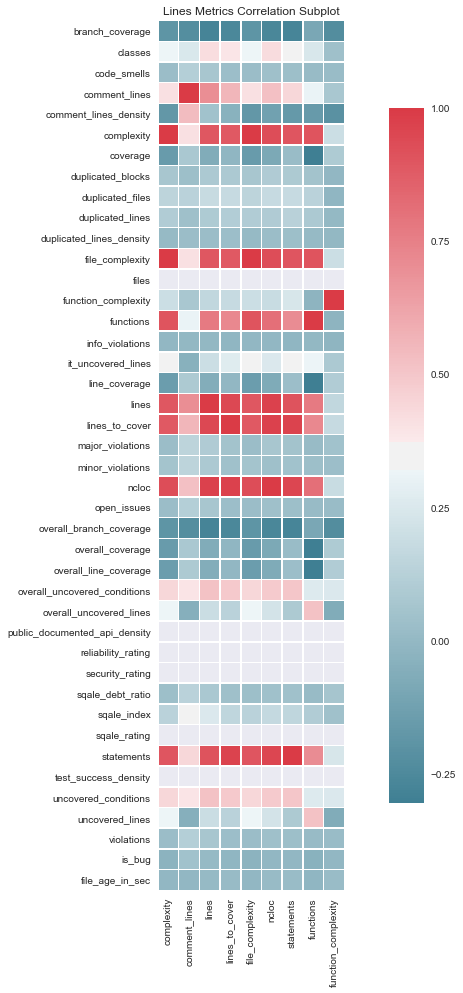
\includegraphics[scale=0.7]{\figCorrPath/Lines_Metrics_Correlation_Subplot.png}
    \caption{Line Metrics Correlation Subplot}
    \label{fig:correlation-line-metrics-subplot}
\end{figure}

\begin{figure}[!h]
    \centering
    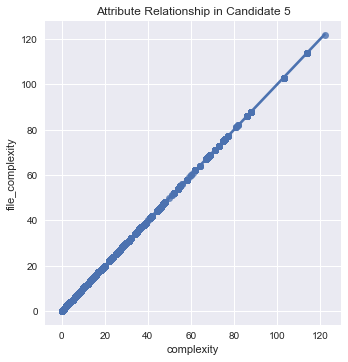
\includegraphics[scale=0.7]{Figures/correlation/Attribute_Relationship_in_Candidate_5.png}
    \caption{Relationship between \complexity{} and \fileComplexity{} attributes}
    \label{fig:candidate5-pairplot}
\end{figure}

\begin{figure}[!h]
    \centering
    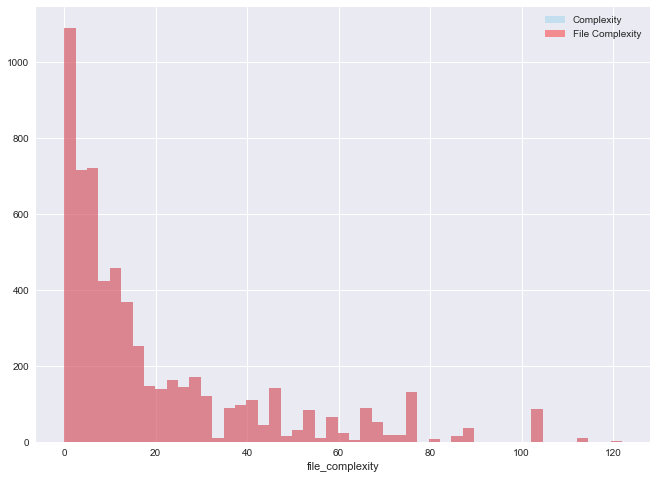
\includegraphics[scale=0.6]{Figures/correlation/Attribute_Distribution_in_Candidate_5.png}
    \caption{Distribution of \complexity{} and \fileComplexity{} Attributes}
    \label{fig:candidate5-distribution}
\end{figure}

For Candidate 6, \statements{} and \linesToCover{}, displayed in Figure \ref{fig:candidate6-scatterplot}, the relationship between them is again distinctly linear, while the distribution, as per Figure \ref{fig:candidate6-distribution} is similar with again a pronounced left tail. 

\begin{figure}[!h]
    \centering
    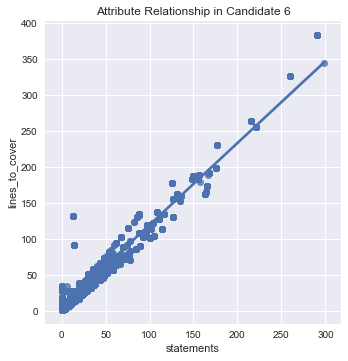
\includegraphics[scale=0.7]{Figures/correlation/Attribute_Relationship_in_Candidate_6.png}
    \caption{Relationship between \statements{} and \linesToCover{} Attributes}
    \label{fig:candidate6-scatterplot}
\end{figure}

\begin{figure}
    \centering
    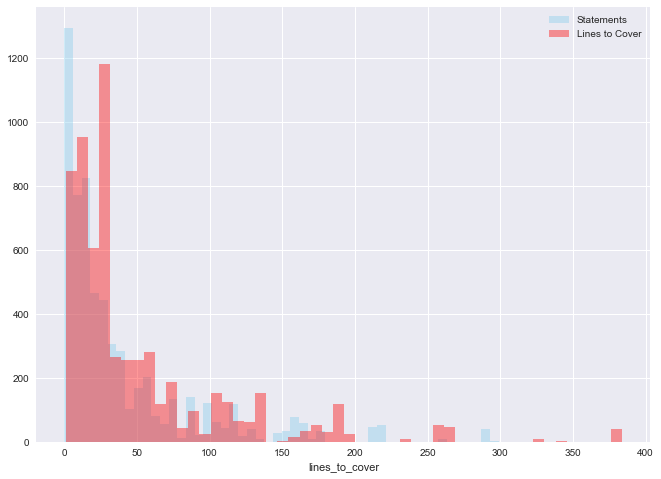
\includegraphics[scale=0.6]{Figures/correlation/Attribute_Distribution_in_Candidate_6.png}
    \caption{Distribution of \statements{} and \linesToCover{} Attributes}
    \label{fig:candidate6-distribution}
\end{figure}

In the next feature transformation candidate, numbered seventh, the relationship between \ncloc{} and \lines{} attributes is again quite linear, as per Figure \ref{fig:candidate7-scatterplot}. From the distribution of the attributes, displayed in Figure \ref{fig:candidate7-distribution} it can be concluded that they follow the distinctly similar pattern.

\begin{figure}
    \centering
    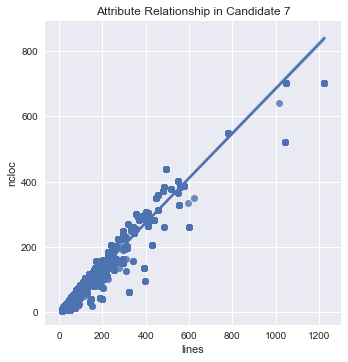
\includegraphics[scale=0.7]{Figures/correlation/Attribute_Relationship_in_Candidate_7.png}
    \caption{Relationship between \ncloc{} and \lines{} Attributes}
    \label{fig:candidate7-scatterplot}
\end{figure}

\begin{figure}
    \centering
    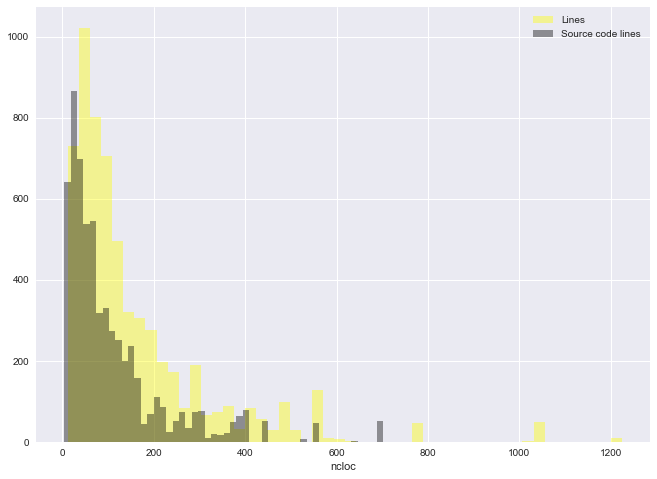
\includegraphics[scale=0.6]{Figures/correlation/Attribute_Distribution_in_Candidate_7.png}
    \caption{Distribution of \ncloc{} and \lines{} Attributes}
    \label{fig:candidate7-distribution}
\end{figure}


In order to further the analysis of the candidates, given the high correlation between a number of features, a number of three-dimensional plots were developed. They serve to better illustrate the relationship between multiple attributes at a time than multiple two-dimensional plots.

From Figure \ref{fig:3d:ncloc-linesToCover-statements} it can be observed that there is an almost perfect linear relationship between \statements{}, \ncloc{} and \lines{} attributes- and this stands to reason as all three metrics would be used to describe source code, with the distinction of \lines{} attribute covering both comment and source code lines in any file. This relationship can also be viewed in Figure \ref{fig:3d:statements-lines-commentLines}, where it can be observed that the higher the number of lines the higher the number of both \statements{} and \commentLines{}. The divergence of a small portion of \lines{} attribute from the main graph line is attributed to a growing number of comment lines in the code as opposed to source ones, as covered by \statements{}. This divergence points to different regression lines for \lines{} vs\commentLines{} as well as \lines{} and \statements{}, therefore those 3 are not equivalent and will not be folded up into a single metric.
\begin{figure}[!h]
    \centering
    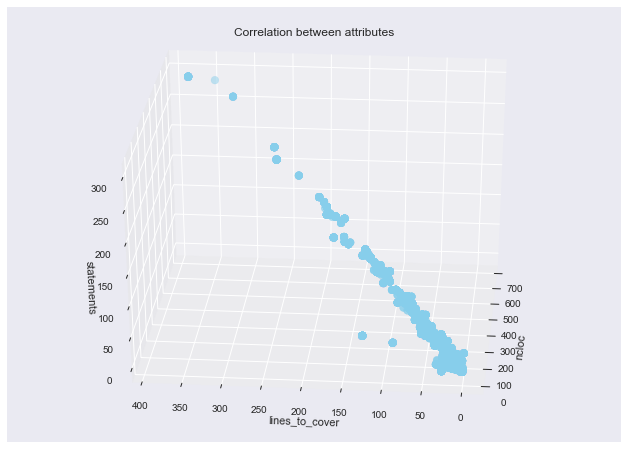
\includegraphics[scale=0.65]{Figures/three-d/Correlation-between-attributes-ncloc-lines_to_cover-statements.png}
    \caption{Relationship between multiple attributes}
    \label{fig:3d:ncloc-linesToCover-statements}
\end{figure}

\begin{figure}[!h]
    \centering
    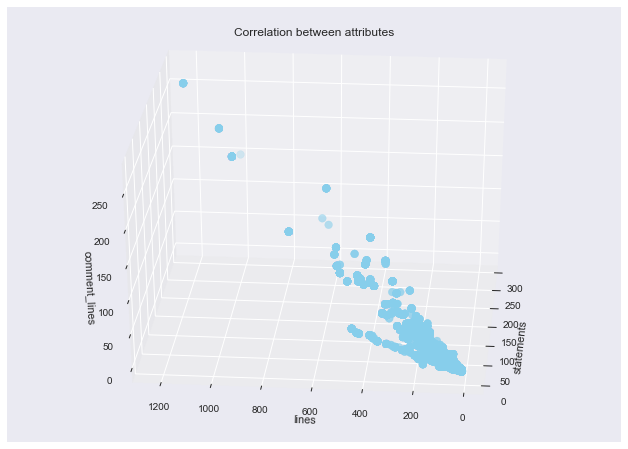
\includegraphics[scale=0.65]{Figures/three-d/Correlation-between-attributes-statements-lines-comment_lines.png}
    \caption{Relationship between multiple attributes}
    \label{fig:3d:statements-lines-commentLines}
\end{figure}

In the exploration of the trends, a plot depicting the relationship between \lines{}, \fileComplexity{} and \commentLines{} has been devised, as it is commonly thought that the more complex the code the more lines of comments and other documentation should be encountered. The results can be seen in Figure \ref{fig:3d:fileComplexity-lines-commentLines} and from the dataset gathered it looks that the hypothesis holds true, there is a correlation between the complexity of a file, its size in absolute terms - represented in the \lines{} attribute, and the number of comments in a given file. 
However, while the trend is present, those metrics are not equivalent and it has been decided against combining them into a single metric.
\begin{figure}[!h]
    \centering
    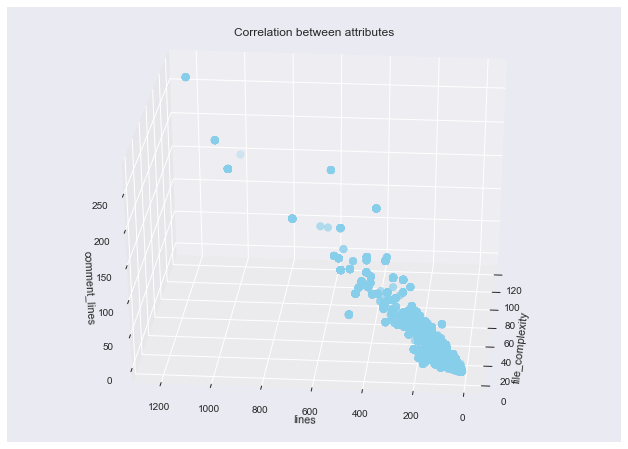
\includegraphics[scale=0.65]{Figures/three-d/Correlation-between-attributes-file_complexity-lines-comment_lines.png}
    \caption{Relationship between multiple attributes}
    \label{fig:3d:fileComplexity-lines-commentLines}
\end{figure}

\FloatBarrier
\textbf{In Conclusion} from the features listed at the beginning of this section it has been sufficiently determined that the following pairs can be safely transformed into a single feature:
\begin{itemize}
    \item \complexity{} and \fileComplexity{} - linear relationship and similar looking distribution
    \item \statements{} and \linesToCover{} - linear relationship and approximately the same distribution
    \item \lines{} and \ncloc{} quite a linear relationship, similar distribution between all.
\end{itemize}

The \complexity{}, \linesToCover{} and \ncloc{} have been retained while their corresponding pairs have been removed from further analysis.
\FloatBarrier
%%%%%%%%%%%%%%%%%%%%%%%%%%%%%%%%%%%%%%%%%%%%%%%%%%%%%%%%%%%%%%%%%%%%%%%%%%%%%%%%%%%%%%%%%%%%%%%%%
\paragraph{Sonar Violation Metrics}\label{sec:impl-data-analysis:corr:sonar-violations}
\begin{figure}[!h]
    \centering
    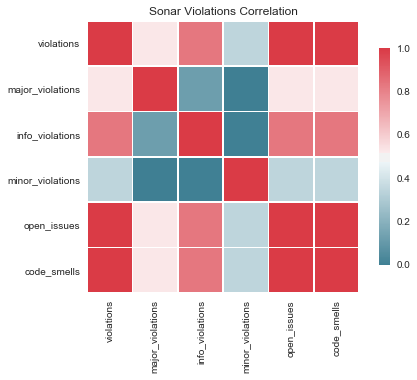
\includegraphics[scale=0.7]{Figures/correlation/Sonar_Violations_Correlation.png}
    \caption{Sonar Violation Metrics Correlation Subplot}
    \label{fig:correlation-sonar-violation-metrics-subplot}
\end{figure}

The following section will investigate if the following candidates can be transformed as per Figure \ref{fig:correlation-sonar-violation-metrics-subplot} there is a strong positive correlation between them:
\resume{enumerate}
    \item \openIssues{}, \violations{} and \codeSmells{}
    \item \majorViolations{}, \minorViolations{} and \infoViolations{}
\suspend{enumerate}

Starting with Candidate 8, the relationship between the attributes appears to be a strong linear one, as can be observed in Figure \ref{fig:3d:candidate8-relationship}. Unfortunately, despite the indications of a strong relationship, there aren't enough data points available to prove it beyond any doubt. The distribution graph, in Figure \ref{fig:candidate8-distribution}, however, clearly states that the distribution of whatever little data points that are available matches perfectly between the three attributes.

\begin{figure}
    \centering
    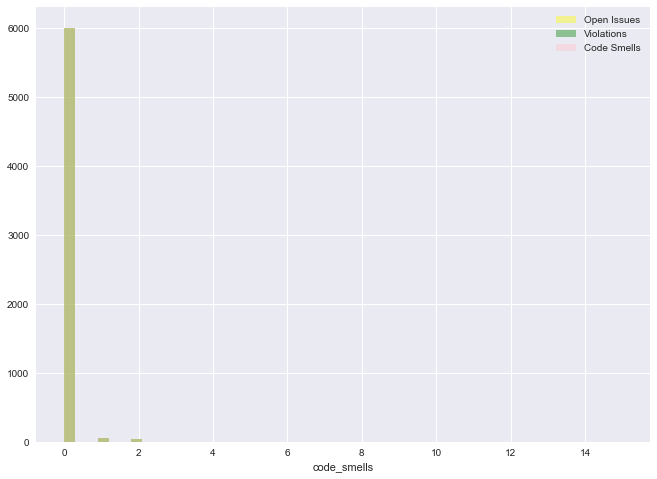
\includegraphics[scale=0.6]{Figures/correlation/Attribute_Distribution_in_Candidate_8.png}
    \caption{Distribution of attributes in Candidate 8}
    \label{fig:candidate8-distribution}
\end{figure}

\begin{figure}[!h]
    \centering
    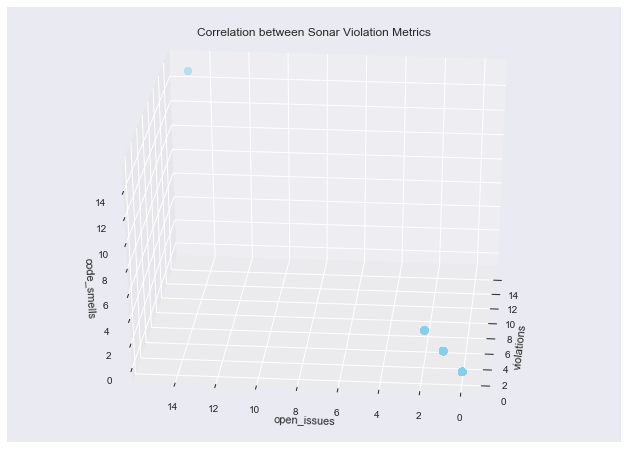
\includegraphics[scale=0.6]{Figures/three-d/Correlation_between_attributes_violations_open_issues_code_smells.png}
    \caption{Correlation between Sonar violation attributes}
    \label{fig:3d:candidate8-relationship}
\end{figure}

\begin{figure}[!h]
    \centering
    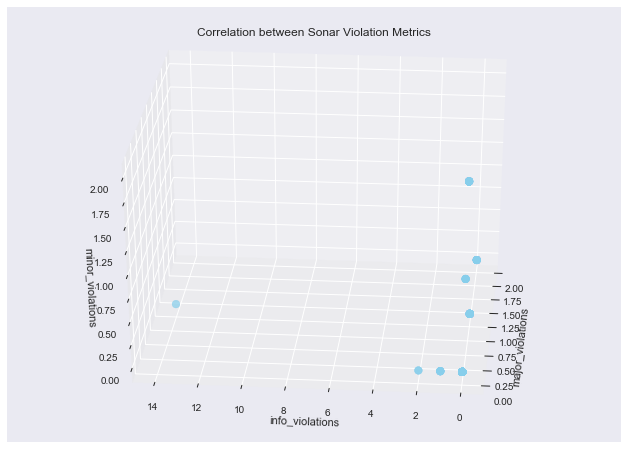
\includegraphics[scale=0.6]{Figures/three-d/Correlation_between_attributes_major_violations_info_violations_minor_violations.png}
    \caption{Correlation between Sonar violation attributes}
    \label{fig:3d:candidate9-relationship}
\end{figure}

\begin{figure}
    \centering
    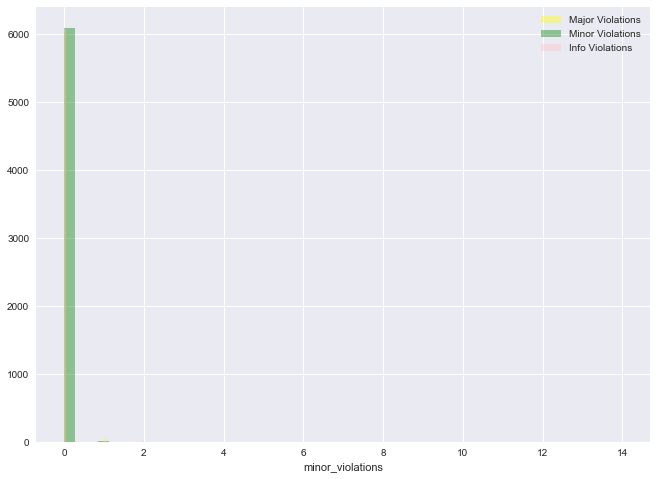
\includegraphics[scale=0.6]{Figures/correlation/Attribute_Distribution_in_Candidate_9.png}
    \caption{Distribution of attributes in candidate 9}
    \label{fig:candidate9-distribution}
\end{figure}

\textbf{In conclusion} the \openIssues{}, \codeSmells{} and \violations{} features can be transformed into a single feature as they show an indication of a linear relationship and have an identical distribution. As such \violations{} feature will be retained while the other 2 will be dropped from the analysis.

A conclusion with regards to remaining metrics is that no strong opportunity for transformation presented itself as there is little defined relationship between the attributes. Furthermore, based on domain knowledge of \infoViolations{}, \minorViolations{} and \majorViolations{} it is concluded that those metrics are independent of one another. 

However, when drawing from the domain knowledge of Sonar metrics, \violations{} is an all-encompassing term used for describing any infraction against rules defined as part of the analysis, such as that depicted by \infoViolations{}, \minorViolations{} or \majorViolations{}. As such, it is natural that \violations{} attribute will be closely related to those metrics. Therefore, the only violation describing metric retained will be \violations{}.
% \FloatBarrier

\paragraph{Code Duplication Metrics}\label{sec:impl-data-analysis:corr:code-duplication}
\begin{figure}
    \centering
    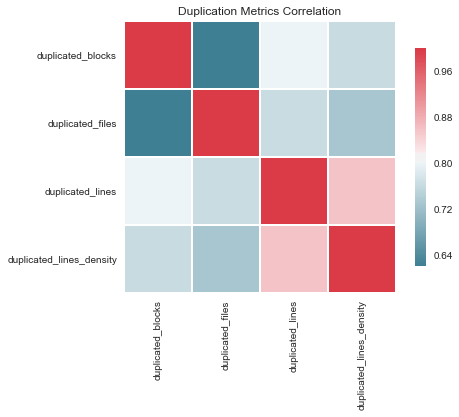
\includegraphics[scale=0.75]{Figures/correlation/Duplication_Metrics_Correlation.png}
    \caption{Code Duplication Metrics Correlation Subplot}
    \label{fig:correlation-code-duplication-metrics-subplot}
\end{figure}
Based on the correlation graph for code duplication metrics the following candidate has been chosen for the analysis:
\resume{enumerate}
    \item \duplicatedBlocks{}, \duplicatedFiles{}, \duplicatedLines{} and \duplicatedLinesDensity{}
\end{enumerate}

\begin{figure}
    \centering
    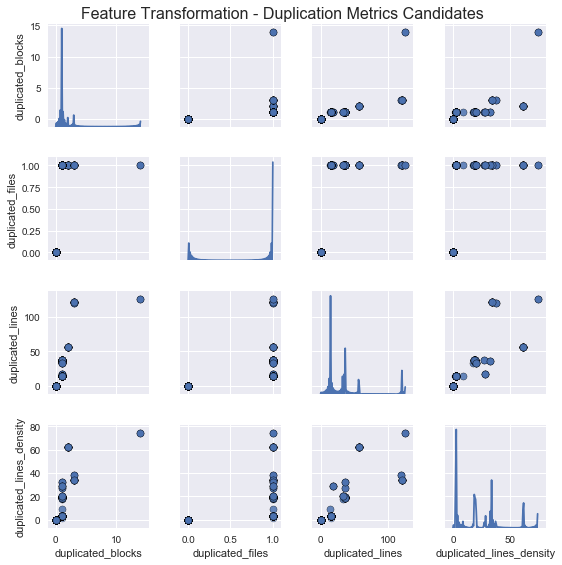
\includegraphics[scale=0.75]{Figures/correlation/Attribute_Relationship_in_Duplication_Metrics.png}
    \caption{Code Duplication Metrics Correlation Subplot}
    \label{fig:correlation-code-duplication-metrics-subplot}
\end{figure}


\textbf{In conclusion} no strong opportunity for transformation has been found between code duplication metrics as the correlation appears to be of small magnitude. The only exception has been displayed by \duplicatedBlocks{} and \duplicatedFiles{} features that showed a strong negative correlation.
\FloatBarrier

\subsubsection{Addressing High Variance in Dataset}\label{sec:impl-data-analysis:dealing-with-variance}
This section is intended to evaluate the variance in the dataset with subsequent subsections evaluating different ways of dealing with high variance features by scaling features to the same order of magnitude.
\subsubsection{Feature Distribution}\label{sec:impl-data-analysis:feature-dist}
\todo{fill it out}
\subsubsection{Outliers}\label{sec:impl-data-analysis:outliers}
The underlying section will look into the number of outliers in the dataset. Given that the linear models, such as logistic regression one can be highly susceptible to the presence of outlying data points this part of the data analysis must be carried out.

Outliers, also referred to as residuals, are the data points not residing on a given prediction function. The magnitude of a residual is typically defined as the distance of a given data point from the proposed prediction line, in linear models.

Taking into the account the number of features present in the dataset it would be quite unfeasible to present individual box plot graphs per feature. At the same time, since the data is not yet on the same scale it would be difficult to highlight any residuals on aggregate graphs, with multiple features on each plot. Therefore it was decided that an algebraic method will be best employed instead.

The first step was to collect the following properties for each feature:
\begin{itemize}
    \item first quartile (Q1)
    \item third quartile (Q3)
    \item interquartile range (IQR)
    \item lower boundary - value below which a data point will be considered an outlier. Set to $1.5x IQR$ below the first quartile
    \item upper boundary - value above which a data point will be considered an outlier. Set to $1.5x IQR$ above third quartile
\end{itemize}

The above metrics are collected into a list. Each list item is a map of an attribute to value. The information collected was then converted to a data frame for enabling easy processing. The results compiled can be observed in Tables \ref{tbl:outliers:iqr-at-0} and \ref{tbl:outliers:all-metrics}.

\begin{table}[!h]
\centering
\caption{All metrics pertaining to calculating residuals - IQR at 0}
\label{tbl:outliers:iqr-at-0}
\begin{tabular}{@{}lll@{}}
\toprule
\multicolumn{3}{c}{Feature Names} \\ \midrule
duplicated\_blocks & major\_violations & reliability\_rating \\
duplicated\_files & minor\_violations & security\_rating \\
duplicated\_lines & overall\_branch\_coverage & sqale\_debt\_ratio \\
duplicated\_lines\_density & overall\_coverage & sqale\_index \\
files & overall\_uncovered\_conditions & sqale\_rating \\
info\_violations & overall\_uncovered\_lines & test\_success\_density \\
it\_uncovered\_lines & public\_documented\_api\_density & violations \\ \bottomrule
\end{tabular}
\end{table}

\begin{table}[!h]
\centering
\caption{All metrics pertaining to calculating residuals - IQR above 0}
\label{tbl:outliers:all-metrics}
\begin{tabular}{@{}llllll@{}}
\toprule
Attribute & IQR & \begin{tabular}[c]{@{}l@{}}Lower \\ Boundary\end{tabular} & Q1 & Q3 & \begin{tabular}[c]{@{}l@{}}Upper \\ Boundary\end{tabular} \\ \midrule
classes & 1 & 0 & 0 & 1 & 2.5 \\
comment\_lines & 15 & 0 & 1 & 16 & 38.5 \\
comment\_lines\_density & 17.8 & 0 & 0.4 & 18.2 & 44.9 \\
complexity & 23 & 0 & 3 & 26 & 60.5 \\
function\_complexity & 0.7 & 0 & 1 & 1.7 & 2.75 \\
functions & 14 & 0 & 3 & 17 & 38 \\
lines\_to\_cover & 44 & 0 & 14 & 58 & 124 \\
ncloc & 105 & 0 & 32 & 137 & 294.5 \\
file\_age\_in\_sec & 87187 & 0 & 3423 & 90610 & 221390.5 \\ \bottomrule
\end{tabular}
\end{table}

Subsequently, it is checked which columns contain values above their upper outlier boundary. Another list containing the columns without residuals above such value is also compiled. 

At the end of that process, it has been concluded that 22 columns contain residuals while 8 do not. Furthermore, counts of residual data points have been obtained and compiled into Table \ref{tbl:outliers:counts-original}. The items in yellow, have been highlighted to signify their $IQR$ value being above 0. From same it can be observed that the most significant numbers of residual data points is observed in \itUncoveredLines{}, closely followed by \overallUncoveredLines{}, \fileAgeInSec{} and \overallUncoveredConditions{} attributes. However, other than \fileAgeInSec{} other mentioned attributes have their $IQR$ value at 0, as per lack of the yellow highlight and given values contained in Table \ref{tbl:outliers:iqr-at-0}, meaning any data points above that value would automatically be treated as an outlier. Judging by Table \ref{tbl:outliers:all-metrics} the attributes are of similar enough scale to be grouped together for visualization, the result of which can be observed from Figures \ref{fig:outliers:boxplot-iqr-above-0-part1} and \ref{fig:outliers:boxplot-iqr-above-0-part2}. 

\begin{table}[!h]
\centering
\caption{Residual counts per feature}
\label{tbl:outliers:counts-original}
\begin{tabular}{ll}
\hline
Column & \begin{tabular}[c]{@{}l@{}}Data Points Above \\ Upper Boundary\end{tabular} \\ \hline
\rowcolor[HTML]{FFFFC7} 
classes & 534 \\
\rowcolor[HTML]{FFFFC7} 
comment\_lines & 797 \\
\rowcolor[HTML]{FFFFC7} 
comment\_lines\_density & 359 \\
\rowcolor[HTML]{FFFFC7} 
complexity & 491 \\
duplicated\_blocks & 221 \\
duplicated\_files & 221 \\
duplicated\_lines & 221 \\
duplicated\_lines\_density & 221 \\
\rowcolor[HTML]{FFFFC7} 
file\_age\_in\_sec & 985 \\
\rowcolor[HTML]{FFFFC7} 
function\_complexity & 294 \\
\rowcolor[HTML]{FFFFC7} 
functions & 462 \\
info\_violations & 11 \\
it\_uncovered\_lines & 1100 \\
\rowcolor[HTML]{FFFFC7} 
lines\_to\_cover & 652 \\
major\_violations & 70 \\
minor\_violations & 24 \\
\rowcolor[HTML]{FFFFC7} 
ncloc & 492 \\
overall\_uncovered\_conditions & 873 \\
overall\_uncovered\_lines & 1087 \\
sqale\_debt\_ratio & 96 \\
sqale\_index & 96 \\
violations & 103 \\ \hline
\end{tabular}
\end{table}

\begin{figure}[!h]
    \centering
    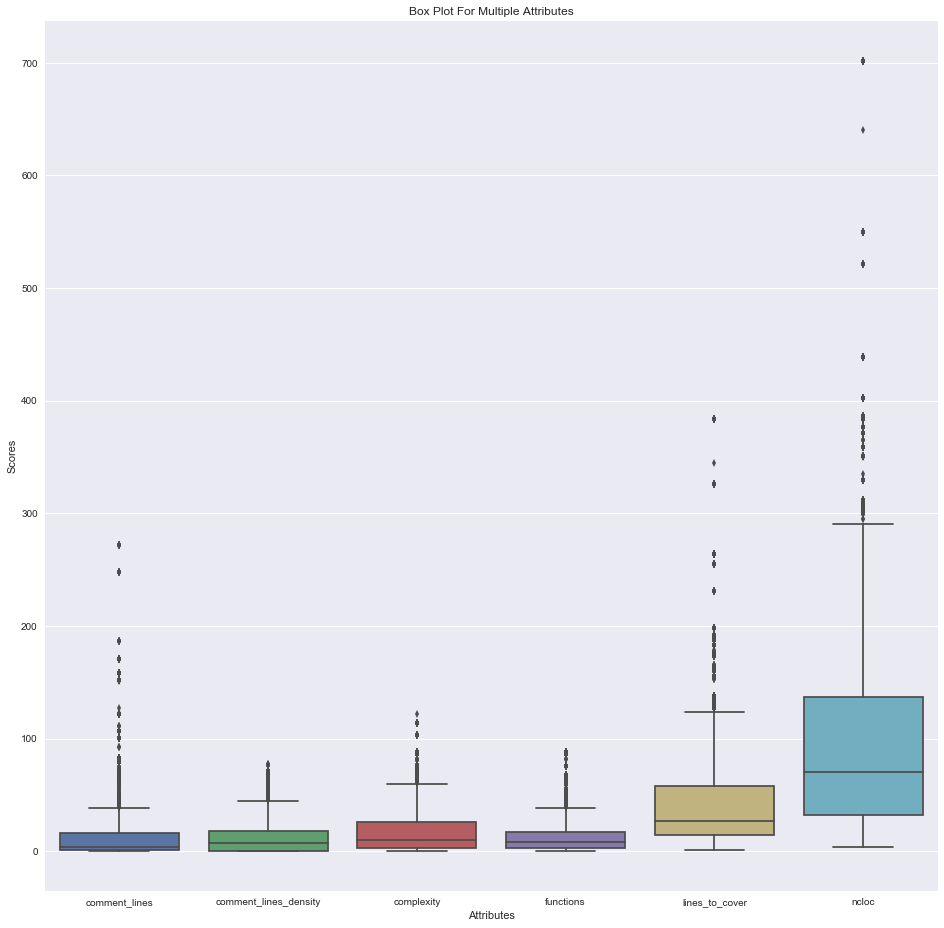
\includegraphics[scale=0.45]{Figures/boxplot_iqr_above_0_part1.png}
    \caption{Residual values for attributes with IQR > 0}
    \label{fig:outliers:boxplot-iqr-above-0-part1}
\end{figure}

\begin{figure}[!h]
    \centering
    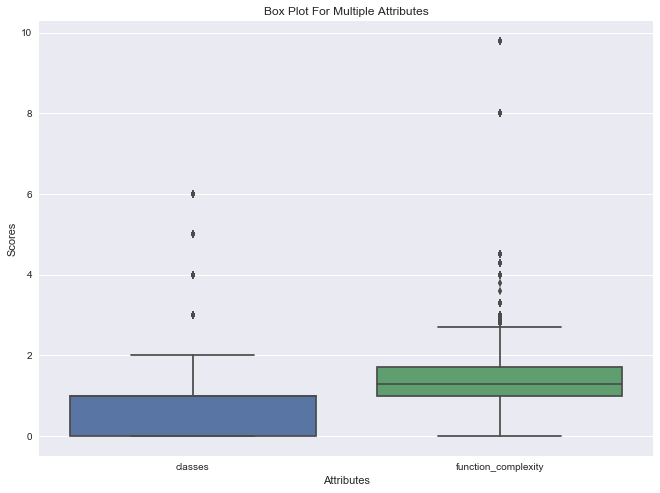
\includegraphics[scale=0.65]{Figures/boxplot_iqr_above_0_part2.png}
    \caption{Residual values for attributes with IQR > 0}
    \label{fig:outliers:boxplot-iqr-above-0-part2}
\end{figure}

\textbf{In Conclusion} it has been proven beyond any doubt that there are a number of outliers in the dataset. At this stage, it has been decided against addressing the residual values as it will undergo further processing with regards to scaling as well as due to recognizing that only 1 of the machine learning models used, logistic regression, is susceptible to their presence. 
\FloatBarrier
\subsubsection{Addressing High Variance in Dataset}\label{sec:impl-data-analysis:dealing-with-variance}
This section is intended to evaluate the variance in the dataset with subsequent subsections evaluating different ways of mitigating the high variance features by scaling features to the same order of magnitude.

The first method utilized was using natural logarithm $log(e)$, which was conducted in steps described in detail as follows.
\paragraph{$log(e)$ - Determining which columns to scale}
First, the dataset was copied in order to avoid polluting the original dataset. Then in order to ensure that all values are on approximately the same scale a list of columns where column variance was above the third quartile of the overall variance values was compiled. 

The third quartile for the variance of the dataset was calculated by first finding variance for each column, using \texttt{var()} function available on DataFrame all objects. The resulting data series, with its rows corresponding to the variance value of a given feature and a single column where the actual value is contained, was converted to a data frame and passed to the \texttt{collect\_outlier\_data\_to\_list} function. Said function is responsible for calculating the following metrics for a given set of data provided to it:

\begin{itemize}
    \item first quartile (Q1)
    \item third quartile (Q3)
    \item interquartile range (IQR)
    \item lower outlier boundary - value below which a data point will be considered an outlier. Set to $1.5x IQR$ below the first quartile
    \item upper outlier boundary - value above which a data point will be considered an outlier. Set to $1.5x IQR$ above third quartile
\end{itemize}

As a result of the call, the Q3 for the complete variance was calculated and returned for use in the next step.

Given the dataset Q3 value determined, it was possible to iterate over the complete dataset, column by column, verifying that a given column contains only numeric type data, and finally checking if the variance of the feature is above the Q3 threshold specified. If it was, such column was appended to a list, which when iteration was complete was returned. 

The names of columns gathered as a result are presented in Table \ref{tbl:available-data-non-repeating-types}.

\begin{table}[!h]
\centering
\caption{Columns with variance greater than Q3 of overall variance in the dataset}
\label{tab:loge-scaler-cols-aboveq3}
\begin{tabular}{@{}l@{}}
\toprule
Column name \\ \midrule
comment\_lines \\
comment\_lines\_density \\
complexity \\
it\_uncovered\_lines \\
lines\_to\_cover \\
ncloc \\
overall\_coverage \\
file\_age\_in\_sec \\ \bottomrule
\end{tabular}
\end{table}

\paragraph{$log(e)$ - Executing the scaler}
Subsequently \texttt{convert\_col\_vals\_to\_log} function was used to convert values in all columns collected to their natural logarithm representation and subsequently appended to the dataset.

\paragraph{$log(e)$ - Conclusion}
Table \ref{tbl:loge-scaler-cols-transformed} depicts the results of the transformation. While most of the obtained variance values are of a much smaller scale and slightly more in line with the remaining values, given that 75\% of values are below the value of approximately 240, the transformed columns are now undervalued. 
Additionally, the \texttt{nan} values indicate that a number could not be obtained as a result of the transformation, likely due to the too small a value of original variance. 

\textbf{In conclusion} given that not all values are of the same scale at the end of this process, and given the presence of non-numerical values, \texttt{nan}, it has been decided against the usage of natural logarithm scaling method.
\begin{table}[!h]
\centering
\caption{Scaled variance results}
\label{tbl:loge-scaler-cols-transformed}
\begin{tabular}{@{}ll@{}}
\toprule
Column Name & Transformed Variance Value \\ \midrule
comment\_lines\_log & nan \\
comment\_lines\_density\_log & nan \\
complexity\_log & nan \\
it\_uncovered\_lines\_log & 0.23 \\
lines\_to\_cover\_log & 1.23 \\
ncloc\_log & 1.08 \\
overall\_coverage\_log & nan \\
file\_age\_in\_sec\_log & 5.49 \\ \bottomrule
\end{tabular}
\end{table}


\paragraph{Scaling using Sci-Kit Learn's built-in methods}
The following scaling methods will be applied sequentially to all data points subsequently used in the analysis:
\begin{itemize}\label{lst:list-of-scalers}
    \item Min Max, described in section \ref{sec:data-modelling:scalers:min-max}
    \item Max Abs - corresponds to Decimal Scaling method, section \ref{sec:data-modelling:scalers:max-abs}
    \item Standard, corresponds to Z-Score method, section \ref{sec:data-modelling:scalers:standard}
    \item Power Transformer using Yeo-Johnson method, section \ref{sec:data-modelling:scalers:power-yeo-johnson}
    \item Quantile Normal, section \ref{sec:data-modelling:scalers:quantile}
    \item Quantile Uniform, section \ref{sec:data-modelling:scalers:quantile}
\end{itemize}

Data frames containing scaled data will be compiled into a reference map for easy lookup of data.

Following scaled data collection, the standard deviation for each column for each of the methods will be compared to check the data distribution. Decided on a numerical method as compiling graphs for all of 6 scaling methods times 41 features would be inefficient. Graphs may be compiled for illustrating some of the distribution improvements.

Finally, each scaled dataset will be used in Logistic Regression and Decision Tree Algorithm for analysis.

\paragraph{Initial Setup}\label{sec:scalers:initial-setup}
The data scaling operation began by compiling a number of constants holding the designators for each of the methods listed in \ref{lst:list-of-scalers}, the order in which those scaling methods will be executed as well as permanent storage for holding the result of scaling operation on the upsampled and the downsampled datasets.
The order of execution was as follows: min max, decimal scaling, Z-score, Power transformer using Yeo-Johnson method, quantile scaling using normal distribution and lastly quantile scaling using uniform distribution variant.

The last step in the initial setup is to save a copy of the original, unscaled upsampled and downsampled datasets, in their respective storage objects. It is a necessary step in enabling easy comparison of results in due course of the analysis.

\paragraph{Executing Scalers}
Executing and fitting all scalers to the dataset provided has been carried out. However, since scaling methods only apply to the numeric columns, the target column and well as text data columns have been dropped from the scaling operation.

Text columns dropped are pertaining to:
\begin{itemize}
    \item author
    \item previous author
    \item issue key
    \item file path
    \item source repository
\end{itemize}

All of the above have been retained in the dataset only for verification purposes to make sure that any transformed data point can be traced back to its original state.

Subsequently, all scalers are created in the order of their appearance defined in \ref{sec:scalers:initial-setup}. Then they are subsequently executed and fitted to the upsampled and downsampled datasets after which the results are saved in the storage objects for later processing.

\paragraph{Comparing variance change per scaling method}
Following the execution of all scaling methods, it has been deemed necessary to verify if applying various scalers had any effect and investigate what that effect was.

The verification, which is the focus of the underlying section, started with calculating the mean and the median of the standard distribution for each of the scaling methods, per dataset. The results presented in Table \ref{tbl:scalers:mean-and-median-sigma}. It can be clearly observed from there that the standard distribution for the unscaled data, and conversely the variance, is highly skewed with its mean for $\sigma$ being approximately 40 times larger than the median. This trend is observed regardless of the resampling method taken to generate the dataset as it appears in both the upsampled and downsampled datasets. At the same time, the mean and median of standard deviation for any of the scaled dataset are very closely positioned indicating more even distribution of variance across the data points.

\begin{table}[!h]
\centering
\caption{Statistics compiled for scalers}
\label{tbl:scalers:mean-and-median-sigma}
\begin{tabular}{@{}lllll@{}}
\toprule
Method & \begin{tabular}[c]{@{}l@{}}Mean \\ Upsample\end{tabular} & \begin{tabular}[c]{@{}l@{}}Mean \\ Downsample\end{tabular} & \begin{tabular}[c]{@{}l@{}}Median \\ Upsample\end{tabular} & \begin{tabular}[c]{@{}l@{}}Median \\ Downsample\end{tabular} \\ \midrule
Unscaled & 162304.03 & 149887.74 & 3792.53 & 522.45 \\
Min-Max & 3794.98 & 524.61 & 3794.99 & 524.62 \\
Max-Abs & 3794.92 & 524.55 & 3794.96 & 524.59 \\
Standard & 3792.15 & 521.95 & 3794.47 & 524.13 \\
\begin{tabular}[c]{@{}l@{}}Power: \\ Yeo-Johnson\end{tabular} & 3794.89 & 524.53 & 3794.96 & 524.59 \\
\begin{tabular}[c]{@{}l@{}}Quantile:\\ Normal Distribution\end{tabular} & 3795.66 & 525.3 & 3795.98 & 525.62 \\
\begin{tabular}[c]{@{}l@{}}Quantile:\\ Uniform Distribution\end{tabular} & 3794.95 & 524.58 & 3794.98 & 524.61 \\ \bottomrule
\end{tabular}
\end{table}

Variance data for all scaling methods have been compiled into a single dataset for easy manipulation and visualization. In the below Table \ref{tbl:scalers:summary-variance-per-scaler} it can be observed that in the case of the dataset in question applying any scaling method decreased data variance metric significantly.

However, Table \ref{tbl:scalers:summary-variance-per-scaler} fails to intuitively illustrate the distribution of said variance across scalers applied. To better demonstrate that point a number of bar plots have been generated depicting the variance per column, per each scaler for both upsampled and downsampled datasets. 

It should be noted that only a subset of the graph has been presented as significant similarities have been discovered between some methods, with min-max and max-abs scalers producing almost the same looking variance plots, both quantile scalers as well as standard, or Z-score, scaler also producing extremely similar graphs.

Furthermore, when visualizing variance, as per implementation listed in code snippet \ref{code:charting-variance-post-resample}, the \fileAgeInSec{} feature has been removed as its extreme value was overshadowing all other variance metrics making them appear the same in magnitude. 

\begin{landscape}
\begin{table}[!h]
\centering
\caption{Variance summary per column per scaler}
\label{tbl:scalers:summary-variance-per-scaler}
\begin{tabular}{@{}llllllll@{}}
\toprule
 & Max-Abs & Min-Max & \begin{tabular}[c]{@{}l@{}}Power:\\ Yeo-Johnson\end{tabular} & \begin{tabular}[c]{@{}l@{}}Quantile:\\ Normal\\ Distribution\end{tabular} & \begin{tabular}[c]{@{}l@{}}Quantile:\\ Uniform\\ Distribution\end{tabular} & Standard & Unmodified \\ \midrule
classes & 0.03 & 0.03 & 1.00 & 7.26 & 0.10 & 1.00 & 1.01 \\
comment\_lines & 0.02 & 0.02 & 1.00 & 6.10 & 0.11 & 1.00 & 1241.19 \\
comment\_lines\_density & 0.04 & 0.04 & 1.00 & 6.14 & 0.11 & 1.00 & 228.09 \\
complexity & 0.04 & 0.04 & 1.00 & 2.54 & 0.09 & 1.00 & 493.30 \\
duplicated\_blocks & 0.00 & 0.00 & 1.00 & 2.41 & 0.04 & 1.00 & 0.37 \\
duplicated\_files & 0.04 & 0.04 & 1.00 & 4.80 & 0.04 & 1.00 & 0.04 \\
duplicated\_lines & 0.01 & 0.01 & 1.00 & 2.41 & 0.04 & 1.00 & 129.53 \\
duplicated\_lines\_density & 0.01 & 0.01 & 1.00 & 2.40 & 0.04 & 1.00 & 77.14 \\
files & 0.00 & 0.00 & 0.00 & 0.00 & 0.00 & 0.00 & 0.00 \\
function\_complexity & 0.01 & 0.01 & 1.00 & 2.15 & 0.08 & 1.00 & 0.64 \\
functions & 0.03 & 0.03 & 1.00 & 1.32 & 0.08 & 1.00 & 210.53 \\
info\_violations & 0.00 & 0.00 & 1.00 & 0.45 & 0.01 & 1.00 & 0.14 \\
it\_uncovered\_lines & 0.01 & 0.01 & 1.00 & 1.46 & 0.06 & 1.00 & 1177.56 \\
lines\_to\_cover & 0.02 & 0.02 & 1.00 & 1.19 & 0.08 & 1.00 & 3390.29 \\
major\_violations & 0.01 & 0.01 & 1.00 & 1.54 & 0.02 & 1.00 & 0.04 \\
minor\_violations & 0.00 & 0.00 & 1.00 & 0.50 & 0.01 & 1.00 & 0.01 \\
ncloc & 0.03 & 0.03 & 1.00 & 1.21 & 0.08 & 1.00 & 13495.89 \\
overall\_branch\_coverage & 0.00 & 0.00 & 1.00 & 5.97 & 0.11 & 1.00 & 29.33 \\
overall\_coverage & 0.03 & 0.03 & 1.00 & 9.08 & 0.15 & 1.00 & 298.15 \\
overall\_uncovered\_conditions & 0.03 & 0.03 & 1.00 & 6.32 & 0.11 & 1.00 & 2.05 \\
overall\_uncovered\_lines & 0.01 & 0.01 & 1.00 & 6.65 & 0.12 & 1.00 & 95.00 \\
public\_documented\_api\_density & 0.00 & 0.00 & 0.00 & 0.00 & 0.00 & 0.00 & 0.00 \\
reliability\_rating & 0.00 & 0.00 & 0.00 & 0.00 & 0.00 & 0.00 & 0.00 \\
security\_rating & 0.00 & 0.00 & 0.00 & 0.00 & 0.00 & 0.00 & 0.00 \\
sqale\_debt\_ratio & 0.00 & 0.00 & 1.00 & 1.57 & 0.03 & 1.00 & 0.10 \\
sqale\_index & 0.01 & 0.01 & 1.00 & 1.56 & 0.03 & 1.00 & 205.75 \\
sqale\_rating & 0.00 & 0.00 & 0.00 & 0.00 & 0.00 & 0.00 & 0.00 \\
test\_success\_density & 0.00 & 0.00 & 0.00 & 0.00 & 0.00 & 0.00 & 0.00 \\
violations & 0.00 & 0.00 & 1.00 & 1.78 & 0.03 & 1.00 & 0.22 \\
file\_age\_in\_sec & 0.00 & 0.00 & 1.00 & 1.02 & 0.08 & 1.00 & 232942635109.04 \\ \bottomrule
\end{tabular}
\end{table}
\end{landscape}

\begin{figure}[!h]
    \centering
    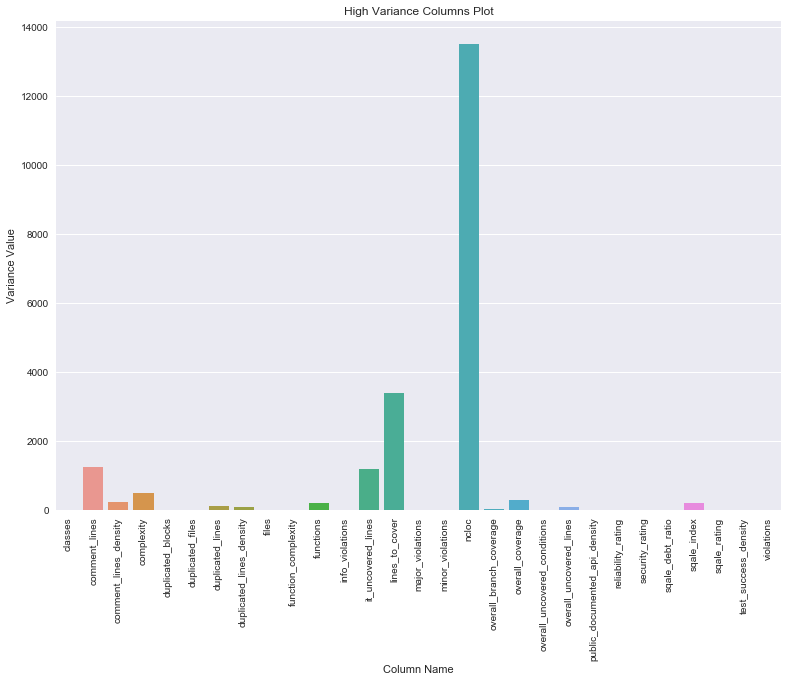
\includegraphics[scale=0.6]{Figures/Variance/downsample/Comparison_of_variance_per_column_for_unmodified_downsampled_dataset.png}
    \caption{Variance per column - No scaler - Downsampled Dataset}
    \label{fig:scalers:variance-unscaled-downsample}
\end{figure}

\begin{figure}[!h]
    \centering
    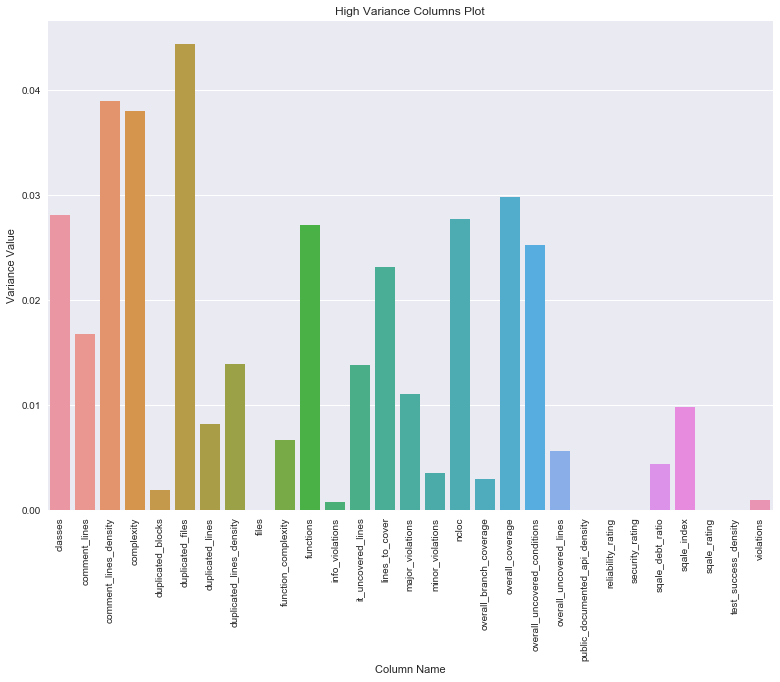
\includegraphics[scale=0.6]{Figures/Variance/downsample/Comparison_of_variance_per_column_for_min-max_downsampled_dataset.png}
    \caption{Variance per column - Min Max scaler - Downsampled Dataset}
    \label{fig:scalers:variance-min-max-downsample}
\end{figure}

\begin{figure}[!h]
    \centering
    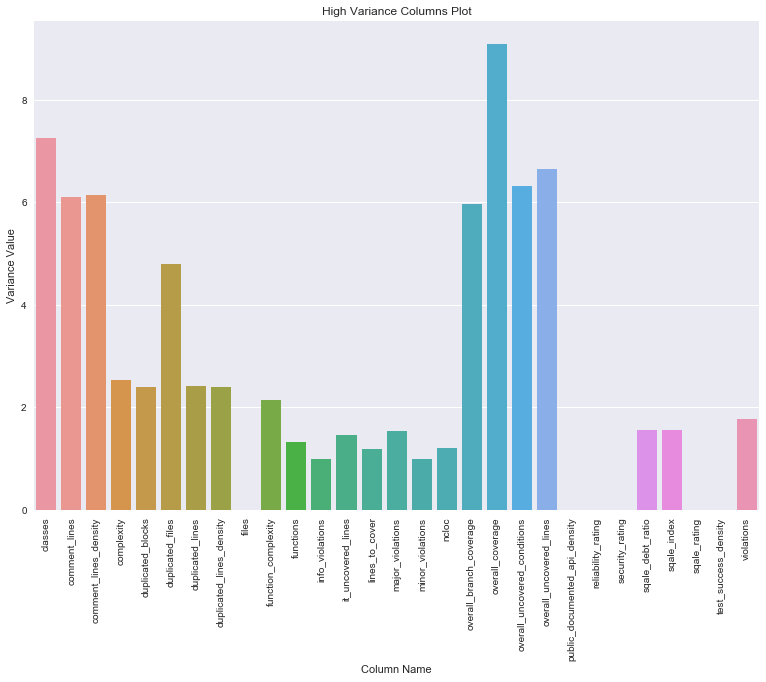
\includegraphics[scale=0.6]{Figures/Variance/downsample/Comparison_of_variance_per_column_for_quantile-normal_downsampled_dataset.png}
    \caption{Variance per column - Quantile scaler with Normal Distribution - Downsampled Dataset}
    \label{fig:scalers:variance-quantile-normal-downsample}
\end{figure}

\begin{figure}[!h]
    \centering
    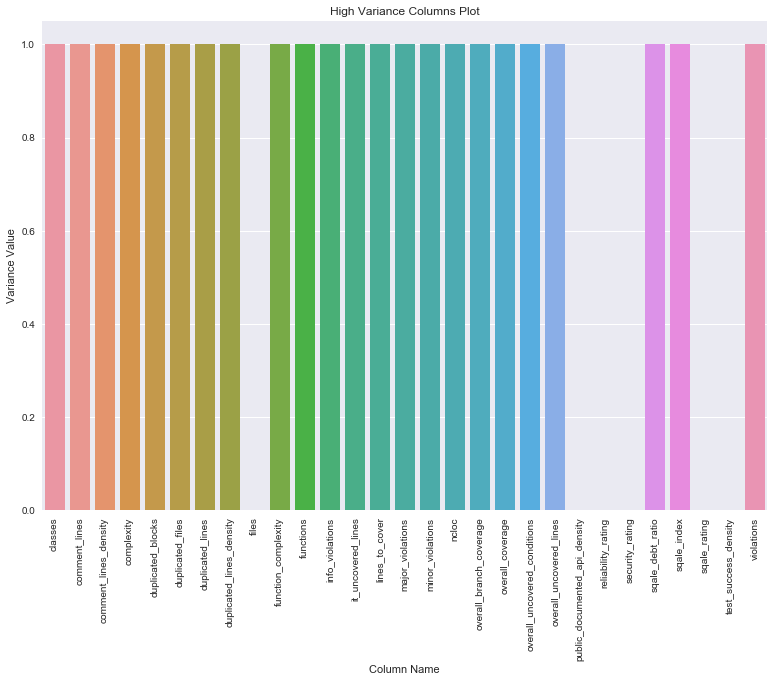
\includegraphics[scale=0.6]{Figures/Variance/downsample/Comparison_of_variance_per_column_for_power-yeo-johnson_downsampled_dataset.png}
    \caption{Variance per column - Power scaler with Yeo-Johnson method - Downsampled Dataset}
    \label{fig:scalers:variance-power-yeo-johnson-downsample}
\end{figure}

Figures \ref{fig:scalers:variance-min-max-downsample}, \ref{fig:scalers:variance-quantile-normal-downsample} and \ref{fig:scalers:variance-power-yeo-johnson-downsample} depict variance per column. By comparing it with the variance of the unscaled dataset, Figure \ref{fig:scalers:variance-unscaled-downsample}, it can be surmised that the data variance has indeed been smoothed out, with power transformer scaler, Figure \ref{fig:scalers:variance-power-yeo-johnson-downsample}, taking on the most extreme case of evening out, where all present variance metrics are equal to 1.
\FloatBarrier

\paragraph{Residuals in scaled datasets}\label{sec:scalers:outliers}
Similarly to the residual value analysis conducted in section \ref{sec:impl-data-analysis:outliers} this section will establish if any residuals have been removed due to the scaling of the data. 

Given the definitions of scalers used, as discussed in section \ref{sec:data-modelling:scalers} it is assumed that the exact same amount of residuals to that displayed in section \ref{sec:impl-data-analysis:outliers} will be present. 

To that effect, metrics describing residual values, as described in section \ref{sec:impl-data-analysis:outliers}, has again been compiled, this time for each dataset generated by a scaler, for both upsampled and downsampled datasets.

Subsequently, the lists generated depicting columns with and without outliers were compared against the baseline values, outlined previously. 

It has been then concluded that in all cases the counts of the residual data points compiled for scaled dataset matched exactly to the baseline. Therefore, as expected, the scaling of data had no effect on the presence of residuals.

\paragraph{Conclusion}\label{sec:scalers:conclusion}
\textbf{In conclusion} using transformation methods described in the overall section was a step necessary to ensure that the data in question is of the same scale. 

\FloatBarrier

\subsubsection{Implementing Logistic Regression}\label{sec:exec:log-reg}

Execution of Logistic Regression model was conducted in a number of steps. First a control analysis was established with the model being run against the unscaled datasets, both the upsampled and the downsampled ones. In each of the model execution the following steps were executed in order:
\begin{itemize}
    \item the dataset is split into the features used for predictions and the target feature to be predicted, $X$ and $y$ respectively
    \item the X  and y are split into the \texttt{train} and \texttt{test} sets. The \texttt{train} subset is used to train the model and the \texttt{test} subset is used to then verify the predictions made using data points previously unseen by the model in question. The split is $75\%$ data points dedicated to the \texttt{train} subset and $25\%$ to the \texttt{test} subset.
    \item the model is created with either L1 or L2 regularization penalty.
    \item model is trained on the training data subset.
    \item coefficients graph generated. This graph provides visual representation as to which features were significant towards predicting the outcome and which were penalized by the regularization algorithm.
    \item model scoring function is executed on the test subset. The scoring function provides a single decimal number between 0 and 1 and represents the mean accuracy of making a correct prediction. 
    \item statistics about the probability of predicting each class are compiled for the data points. Predicting the probability of selection is an important part of the process as it ensures that the classes are applied evenly and to not become unbalanced. The ideal average result for the probability of a data point being classified as either label is $0.5$ or $50\%$.
\end{itemize}

Subsequently, each of the scaled models have been analyzed using the steps outlined and compared. The only difference between running 1 model at a time and that of iterative execution is the additional functionality has been added to plot the model coefficients in their individual graphs. If executed as is, coefficient graphs would have been plotted in the same plane for all scaled datasets, making it hard to determine how each model fared with regards to the regularized feature selection. 

Regularization is applied even at the initial control group as the model implementation used forces it to be specified. In the case of the Logistic Regression model applied via sci-kit learn package the default regularization applied is L2, therefore making it impossible to obtain non-regularized results for that algorithm.



\subsubsection{Implementing Decision Tree classification}
The decision tree model is first executed on the unscaled downsampled and upsampled datasets in order to establish baseline for both datasets when examining the results of the scaled models.

The execution was conducted in the following steps:\
\begin{itemize}
    \item the dataset under analysis is split into the features used for predictions and the target feature to be predicted, $X$ and $y$ respectively.
    \item the $X$ and $y$ are split into the \texttt{train} and \texttt{test} sets. The \texttt{train} subset is used to train the model and the \texttt{test} subset is used to then verify the predictions made using data points previously unseen by the model in question. The split is $75\%$ data points dedicated to the \texttt{train} subset and $25\%$ to the \texttt{test} subset.
    \item the decision tree model is instantiated
    \item the model is trained by fitting the training set 
    \item new unseen data points are simulated using the test subset
    \item Sci-kit Learn's \texttt{accuracy\_score} function is utilized to determine the accuracy of the prediction made using the simulated new data points and the features of the test subset. The result is presented as a floating point number between 0 and 1, with values closer to 1 representing higher accuracy of the model
    \item the result is multiplied by 100 in order to convert it to a $\%$ value.
\end{itemize}

The same steps are conducted for all of the scaled datasets and the final accuracy score, as per method described is presented.

